\documentclass[preprint, 10pt]{elsarticle}

%\usepackage{algorithmic}
%\usepackage{algorithm}
\usepackage{amsfonts}
\usepackage[fleqn,reqno]{amsmath}
\usepackage{amssymb}
%\usepackage{amsthm}
\usepackage[titletoc]{appendix}
\usepackage{array}
%\usepackage{bm}
%\usepackage{caption}
%\usepackage[usenames]{color}
\usepackage{enumitem}
%\usepackage{epsfig}
%\usepackage{fancybox}
\usepackage{filecontents}
\usepackage[top=1.2in,bottom=1.2in,left=1in, right=1in]{geometry}
\usepackage{graphics}
%%\usepackage{ifthen}
\usepackage{lineno}
%\usepackage{mathrsfs}
%\usepackage{mdframed}
%\usepackage{multirow}
%\usepackage{palatino}
%\usepackage{showkeys} %To see the labels for now.  Will remove later
%\usepackage{stmaryrd}
%\usepackage{subfigure}
%\usepackage{paralist}
\usepackage{pgfplots}
%\usepackage{tabularx}
\usepackage{tikz}
\usepackage{todonotes}
\usetikzlibrary{arrows}
\usepackage{comment}

%%%%%%  pdftex  %%%%%%%%%%%%%%%%%%%%%%%%%%%%%%%%%%%%%%%%%%%%%%%%%%%%%%
\usepackage[pagebackref=false,bookmarks=false]{hyperref} 

\hypersetup{
  bookmarksnumbered=true,
  bookmarksopen=false,
  hypertexnames=false,      
  breaklinks=true,          
  unicode=false,
  pdffitwindow=true,        
  pdfnewwindow=true,        
  colorlinks=true,         
  linkcolor=dblue,
  anchorcolor=red,
  citecolor=dorange,
  filecolor=magenta,
  urlcolor=dblue,
  pdfstartview = FitH,
  pdfkeywords = {},
  pdfcreator = {LaTeX with hyperref package}
}



\newcommand{\bd}{{\partial}}
\newcommand{\bigO}{{\mathcal{O}}}
\newcommand{\cc}{{\mathbf{c}}}
\newcommand{\DD}{{\mathcal{D}}}
\newcommand{\eeta}{{\boldsymbol\eta}}
\newcommand{\ff}{{\mathbf{f}}}
\newcommand{\grad}{{\nabla}}
\newcommand{\II}{{\mathbf{I}}}
\newcommand{\iin}{\mathrm{in}}
\newcommand{\llambda}{{\boldsymbol\lambda}}
\newcommand{\nn}{{\mathbf{n}}}
\newcommand{\NN}{{\mathcal{N}}}
\newcommand{\out}{\mathrm{out}}
\newcommand{\rr}{{\mathbf{r}}}
\newcommand{\RR}{{\mathbb{R}}}
\renewcommand{\ss}{{\mathbf{s}}}
\newcommand{\ssigma}{{\boldsymbol\sigma}}
\newcommand{\tar}{\mathrm{tar}}
\newcommand{\uu}{{\mathbf{u}}}
\newcommand{\UU}{{\mathbf{U}}}
\newcommand{\vv}{{\mathbf{v}}}
\newcommand{\xx}{{\mathbf{x}}}
\newcommand{\xxi}{{\boldsymbol{\xi}}}
\newcommand{\yy}{{\mathbf{y}}}

\def\gap{\hspace*{.2in}}

% Derivatives
\newcommand{\pderiv}[2]{\frac{\partial #1}{\partial #2}}
\newcommand{\tderiv}[2]{\frac{d #1}{d #2}}
\newcommand{\ppd}[2]{\frac{\partial^2 #1}{{\partial #2}^2}}

% Nick's commands
\newcommand{\vsp}[1]{\vspace{#1 pc} \noindent}
\newcommand{\abs}[1]{\lvert #1 \rvert}
\newcommand{\mean}[1]{\left< #1 \right>}
\newcommand{\thL}{$\theta$--$L$}
\newcommand{\eps}{\varepsilon}
\newcommand{\Vn}{V_n}
\newcommand{\Vs}{V_s}
\newcommand{\atau}{\abs{\tau}}
\newcommand{\thalpha}{\pderiv{\theta}{\alpha}}
\newcommand{\elfun}{\zeta}
\newcommand{\thhat}{\hat{\theta}}
\newcommand{\Dt}{\Delta t}
\newcommand{\NLterm}{\mathcal{N}}
\newcommand{\Mterm}{\mathcal{M}}
\newcommand{\FourierSum}{ \sum_{k = -N_\iin /2}^{N_\iin /2-1} }
\newcommand{\atausig}{\atau^{(\sigma)}}
\newcommand{\Vnsig}{\Vn^{(\sigma)}}
\newcommand{\Vssig}{\Vs^{(\sigma)}}


\newcommand{\tauD}[1]{\tau_{#1\text{D}}}
\newcommand{\atauD}[1]{\abs{\tau_{#1\text{D}}}}

\begin{document}

\title{Viscous Transport in Eroding Porous Media}


% OTHER TITLE POSSIBILITIES
% ???

\author[SH]{Shang-Huan Chiu}
\author[Nick]{M.~N.~J.~Moore}
\author[Bryan]{Bryan D.~Quaife}

\address[SH]{Department of Scientific Computing, Florida State
University, Tallahassee, FL, 32306.}
\address[Nick]{Department of Mathematics and Geophysical Fluid Dynamics Institute, Florida State University, Tallahassee, FL, 32306.}
\address[Bryan]{Department of Scientific Computing and Geophysical Fluid Dynamics Institute, Florida State University, Tallahassee, FL, 32306.}

\begin{abstract} 
  An abstract
\end{abstract}

\begin{keyword}
  Keyword 1 \sep Keyword 2 \sep Keyword 3 
\end{keyword}

\maketitle

%%%%%%%%%%%%%%%%%%%%%%%%%%%%%%%%%%%%%%%%%%%%%%%%%%%%%%%%%%%%%%%%%%%%%%%
\section{Introduction}
\label{s:intro}
%%%%%%%%%%%%%%%%%%%%%%%%%%%%%%%%%%%%%%%%%%%%%%%%%%%%%%%%%%%%%%%%%%%%%%%
A continuation of the methods paper~\cite{qua-moo2018}.
\paragraph{Governing Equations}
\begin{equation}
\label{eqn:erosionModel}
\begin{split}
  \mu \Delta \uu = \grad p, &\hspace{20pt} \xx \in \Omega, \gap &&\mbox{\em conservation
of momentum}\\
\grad \cdot \uu = 0, &\hspace{20pt} \xx \in \Omega, \gap &&\mbox{\em conservation of mass} \\
\uu = 0, &\hspace{20pt} \xx \in \gamma, \gap &&\mbox{\em no slip on the
bodies} \\
\uu = \UU, &\hspace{20pt} \xx \in \Gamma, \gap &&\mbox{\em outer wall
velocity} \\
\Vn = \CE \, \abs{\tau}, &\hspace{20pt} \xx \in \gamma,
&&\mbox{\em erosion model}.
\end{split}
\end{equation}



%%%%%%%%%%%%%%%%%%%%%%%%%%%%%%%%%%%%%%%%%%%%%%%%%%%%%%%%%%%%%%%%%%%%%%%
\paragraph{Contributions}
\begin{itemize}
  \item Use novel near-singular Barycentric integration scheme for
    Stokes equation outlined in~\cite{bar-wu-vee2015}. (Remember to
    include historically significant reference Shelley
    \cite{baker1986boundary}).  Also need discuss Helsing and Ojala who
    did a similar panel-based quadrature~\cite{hel-oja2008}
  \item Need to compute one additional derivative since we need the
    derivative of the velocity to find the vorticity and stress tensor
  \item Annealing algorithm to create initial body configurations of specified area fraction specified size distribution (NM can do the writing for this).
  \item Tracer trajectories at different time steps
  \item Compute the anomalous diffusion rate using similar techniques as
    the paper with Pietro~\cite{dea-qua-bir-jua2018}
  \item Need a novel way to do time stepping through the complex
    geometry
\end{itemize}

\paragraph{Limitations}
\begin{itemize}
  \item Bodies are still pinned
  \item Bodies are still two dimensional
\end{itemize}

\paragraph{Related Work}

%%%%%%%%%%%%%%%%%%%%%%%%%%%%%%%%%%%%%%%%%%%%%%%%%%%%%%%%%%%%%%%%%%%%%%%
\paragraph{Outline of the Paper}

%%%%%%%%%%%%%%%%%%%%%%%%%%%%%%%%%%%%%%%%%%%%%%%%%%%%%%%%%%%%%%%%%%%%%%%
\section{Boundary Integral Equation Formulation}
\label{s:formulation}
%%%%%%%%%%%%%%%%%%%%%%%%%%%%%%%%%%%%%%%%%%%%%%%%%%%%%%%%%%%%%%%%%%%%%%%
Continuing with our previous work~\cite{qua-moo2018}, we use a
double-layer potential formulation for the velocity $\uu$.  The
double-layer potential is
\begin{align}
  \uu(\xx) = \DDD[\eeta](\xx) = 
    \int_{\bd\Omega} D(\xx,\yy) \eeta(\yy)\, ds_\yy = 
  \frac{1}{\pi}\int_{\bd\Omega} 
    \frac{\rr \cdot \nn}{\rho^2} \frac{\rr \otimes \rr}{\rho^2}
    \eeta(\yy) \, ds_\yy, \quad \xx \in \Omega,
  \label{eqn:stokesDLP}
\end{align}
where $D$ is the kernel of the integral operator, $\rr = \xx - \yy$,
$\rho = \|\rr\|$, $\nn$ is the unit outward normal at $\yy$, and $\eeta$
is an unknown density function.  In Section~\ref{sec:DLPcomplex}, we
show how the Stokes double-layer potential can also be expressed as the
sum of a Laplacian double-layer potential 
\begin{align}
  \DD[\eta](\xx) = \frac{1}{2\pi} \int_{\bd\Omega}
    \frac{\rr \cdot \nn}{\rho^2} \eta(\yy) ds_\yy
\end{align}
and its gradient.  Since the Laplacian double-layer potential can be
written as a Cauchy integral
\begin{align}
  \DD[\eta](\xx) = \Re (v(x)) \quad \text{where} \quad
  v(x) = \frac{1}{2\pi i} \int_{\bd\Omega}
    \frac{\eta(y)}{x - y} \, dy,
  \label{eqn:laplaceComplex}
\end{align}
where $\xx,\yy \in \RR^2$ are identified with the points $x,y \in \CC$,
the Stokes double-layer potential can be written in terms of Cauchy
integrals and its first derivative.  We also require the derivative of
the Stokes double-layer potential which requires the second derivative
of Cauchy integrals.

We will be using quadrature formulae to compute $v$ and its derivatives
that rely on the Cauchy integral theorem.  Since $v$ is holomorphic, its
value only depends on its boundary data.  The boundary data satisfies
the Sokhotski-Plemelj jump relation
\begin{align}
  \label{eqn:SPrelation}
  v(x) = -\frac{1}{2} \eta(x) + \frac{1}{2\pi i} \int_{\bd\Omega}
    \frac{\eta(y)}{x-y}\, dy, \quad x \in \bd\Omega.
\end{align}
Once the boundary data of $v$ is computed, we have
\begin{align}
  \label{eqn:cauchy}
  v(x) = \frac{1}{2\pi i}\int_{\bd\Omega} 
    \frac{v(y)}{y-x} \,dy, \quad
  v'(x) = \frac{1}{2\pi i} \int_{\bd\Omega}
    \frac{v(y)}{(y-x)^2} \, dy, \quad
  v''(x) = \frac{1}{\pi i} \int_{\bd\Omega}
    \frac{v(y)}{(y-x)^3} \, dy.
\end{align}
for $x \in \Omega$.  Since $v(x)$ depends on the density function $\eta
\in \CC$, we use the notation $v[\eta](x)$ to denote the holomorphic
function defined in equation~\eqref{eqn:laplaceComplex}, and the
derivatives are written as $v'[\eta](x)$ and $v''[\eta](x)$.

The Stokes double-layer potential itself can not represent all solutions
of the incompressible Stokes equations.  Therefore, we complete the
integral equation formulation following the work of Power and
Miranda~\cite{pow-mir1987}.  The completion depends on the Stokeslets
and rotlets
\begin{align}
  S[\llambda_\ell,\cc_\ell](\xx) = \frac{1}{4\pi} \left( 
    -\log \rho \II + \frac{\rr \otimes \rr}{\rho^2} \right), \quad
  R[\xi_\ell,\cc_\ell](\xx) = \frac{\rr^\perp}{\rho^2} \xi_\ell,
\end{align}
where $\rr = \xx - \cc_\ell$, $\cc_\ell$ is a point inside the
$\ell^{th}$ eroding body, $\rr^\perp = (r_2,-r_1)$, and $\rho =
\|\rr\|$.  Then, the solution of the Stokes equation is
\begin{align}
  \uu(\xx) = \DDD[\eeta](\xx) + 
    \sum_{\ell=1}^M S[\llambda_\ell,\cc_\ell](\xx) + 
    \sum_{\ell=1}^M R[\xi_\ell,\cc_\ell](\xx),
\end{align}
where the density function, Stokeslets, and rotlets satisfy
\begin{align}
  \ff(\xx) &= -\frac{1}{2}\eeta(\xx) + \DDD[\eeta](\xx) + 
    \sum_{\ell=1}^M S[\llambda_\ell,\cc_\ell](\xx) + 
    \sum_{\ell=1}^M R[\xi_\ell,\cc_\ell](\xx) +
    \NN_0(\eeta](\xx), \quad \xx \in \bd\Omega, \\
  \llambda_\ell &= \frac{1}{2\pi} \int_{\gamma_\ell} 
    \eeta(\yy)\, ds_\yy \quad \ell = 1,\ldots,M, \\
  \xi_\ell &= \frac{1}{2\pi} \int_{\gamma_\ell}
    (\yy - \cc_\ell)^\perp \cdot \eeta(\yy)\, ds_\yy 
    \quad \ell = 1,\ldots,M,
\end{align}
where $\ff$ is the prescribed Dirichlet boundary condition of the
velocity on the outer wall and eroding bodies.

%%%%%%%%%%%%%%%%%%%%%%%%%%%%%%%%%%%%%%%%%%%%%%%%%%%%%%%%%%%%%%%%%%%%%%%
\subsection{Cauchy Integral Representation of the Double-Layer
Potential}
\label{sec:DLPcomplex}
%%%%%%%%%%%%%%%%%%%%%%%%%%%%%%%%%%%%%%%%%%%%%%%%%%%%%%%%%%%%%%%%%%%%%%%
The Stokes double-layer potential~\eqref{eqn:stokesDLP} can be
decomposed as
\begin{equation}
  \label{eqn:Stokes2Laplace}
  \begin{aligned}
    \DDD[\eeta](\xx) &= 
      \frac{1}{2\pi} \int_{\bd\Omega} 
        \frac{\nn}{\rho^2} (\rr \cdot \eeta) \, ds_\yy + 
      \frac{1}{2\pi} \nabla \int_{\bd\Omega}
        \frac{\rr \cdot \nn}{\rho^2} (\yy \cdot \eeta) \, ds_\yy \\
      &- \frac{1}{2\pi} x_1 \nabla \int_{\bd\Omega}
        \frac{\rr \cdot \nn}{\rho^2}\eta_1(\yy) \, ds_\yy -
      \frac{1}{2\pi} x_2 \nabla \int_{\bd\Omega}
        \frac{\rr \cdot \nn}{\rho^2}\eta_2(\yy) \, ds_\yy.
  \end{aligned}
\end{equation}
All these integrals but the first are a gradient of a Laplace layer
potential.  In addition, each component of the first integral can be
written as a Cauchy integral with a complex-valued density
function~\cite{bar-wu-vee2015}.  Therefore, the Stokes double-layer
potential can be written as five Cauchy integrals and their derivatives
with the density functions $\yy \cdot \eeta$, $\eta_1$, and $\eta_2$.
The individual velocity components are
\begin{align}
  \label{eqn:cauchy1}
  u_1(x) &= \Re (v[\tau_1](x)) + \Re (v'[y\cdot\eta](x)) 
           -x_1\Re (v'[\eta_1](x)) - x_2\Re (v'[\eta_2](x)), \\
  u_2(x) &= \Re (v[\tau_2](x)) - \Im (v'[y\cdot\eta](x)) 
       +x_1\Im (v'[\eta_1](x)) + x_2\Im (v'[\eta_2](x)),
\end{align}
where $y \cdot \eta = y_1 \eta_1 + i y_2 \eta_2 \in \CC$, 
\begin{align} 
  \tau_1=(\eta_1+i\eta_2)\frac{\Re(n)}{n}, \quad \text{and} \quad
  \tau_2=(\eta_1+i\eta_2)\frac{\Im(n)}{n},
\end{align}
and $n \in \CC$ is the complex representation of the outward unit normal
$\nn \in \RR^2$

%%%%%%%%%%%%%%%%%%%%%%%%%%%%%%%%%%%%%%%%%%%%%%%%%%%%%%%%%%%%%%%%%%%%%%%
\subsection{Cauchy Integral Representation of the Shear Stress}
%%%%%%%%%%%%%%%%%%%%%%%%%%%%%%%%%%%%%%%%%%%%%%%%%%%%%%%%%%%%%%%%%%%%%%%
To compute the rate of erosion, we must compute the shear stress of the
double-layer potential
\begin{align}
  \tau(\xx) = \left(\nabla \DDD[\eeta](\xx) + 
    \nabla^T \DDD[\eeta](\xx) \right) \nn \cdot \ss,
\end{align} where $\nn$ and $\ss$ are the unit normal and tangent
vectors at $\xx$, respectively.  Each term of the gradient of the
velocity field can be written in terms of Cauchy integrals.  For
example,
\begin{align}
  \pderiv{u_1}{x_2} &= \Re(iv'[\tau_1](x)) + 
      \Re(i v''[y \cdot \eta](x)) -
      x_1\Re(i v''[\eta_1](x))  -
      \Re(v'[\eta_2](x)) - x_2 \Re(iv''[\eta_2](x)) \\
    &= -\Im(v''[\tau_1](x)) - 
      \Im(v''[y \cdot \eta](x)) +
      x_1\Im(v''[\eta_1](x)) -
      \Re(v'[\eta_2](x)) + x_2 \Im(v''[\eta_2](x)).
\end{align}
Similarly, the other three components of $\nabla \DDD[\eeta]$ can be
calculated
\begin{align}
  \pderiv{u_1}{x_1} &= +\Re (v'[\tau_1](x)) + 
    \Re (v''[y\cdot\eta](x)) - \Re (v'[\eta_1](x)) - 
    x_1\Re (v''[\eta_1](x)) - x_2\Re (v''[\eta_2](x)), \\
  \pderiv{u_1}{x_2} &= - \Im (v'[\tau_1](x)) - 
    \Im (v''[y\cdot\eta](x)) + x_1\Im (v''[\eta_1](x)) - 
    \Re (v'[\eta_2](x)) + x_2\Im (v''[\eta_2](x)), \\
  \pderiv{u_2}{x_1} &= +\Re (v'[\tau_2](x)) - 
    \Im (v''[y\cdot\eta](x)) + \Im (v'[\eta_1](x)) +
    x_1\Im (v''[\eta_1](x)) + x_2\Im (v''[\eta_2](x)), \\
  \pderiv{u_2}{x_2} &= -\Im (v'[\tau_2](x)) - 
    \Re (v''[y\cdot\eta](x)) + x_1\Re (v''[\eta_1](x)) +
    \Im (v'[\eta_2](x)) + x_2\Re (v''[\eta_2](x)).
\end{align}

%%%%%%%%%%%%%%%%%%%%%%%%%%%%%%%%%%%%%%%%%%%%%%%%%%%%%%%%%%%%%%%%%%%%%%%
\subsection{Cauchy Integral Representation of the Vorticity}
%%%%%%%%%%%%%%%%%%%%%%%%%%%%%%%%%%%%%%%%%%%%%%%%%%%%%%%%%%%%%%%%%%%%%%%
Having calculated all derivatives of the double-layer potential, the
vorticity can written in terms of Cauchy integrals.  In particular,
\begin{align}
  \omega(x) = \pderiv{u_2}{x_1} - \pderiv{u_1}{x_2} = 
\Re (v'[\tau_2](x)) + \Im (v'[\tau_1](x)) 
 + \Re (v'[\eta_2](x))+ \Im (v'[\eta_1](x)).
\end{align}

%%%%%%%%%%%%%%%%%%%%%%%%%%%%%%%%%%%%%%%%%%%%%%%%%%%%%%%%%%%%%%%%%%%%%%%
\subsection{Cauchy Integral Representation of the Pressure}
%%%%%%%%%%%%%%%%%%%%%%%%%%%%%%%%%%%%%%%%%%%%%%%%%%%%%%%%%%%%%%%%%%%%%%%
The pressure of the double-layer potential is
\begin{align}
  p(\xx) = -\frac{1}{\pi} \int_{\bd\Omega} \frac{1}{\rho^2}
    \left(1 - 2 \frac{\rr \otimes \rr}{\rho^2} \right) \nn
    \cdot \eeta(\yy) \, ds_\yy.
\end{align}




%%%%%%%%%%%%%%%%%%%%%%%%%%%%%%%%%%%%%%%%%%%%%%%%%%%%%%%%%%%%%%%%%%%%%%%
\section{Transport, Tracers, and Tortuosity}
%%%%%%%%%%%%%%%%%%%%%%%%%%%%%%%%%%%%%%%%%%%%%%%%%%%%%%%%%%%%%%%%%%%%%%%
Erosion leads to interesting porous geometries, and we are interested in
characterizing transport in these geometries.  To characterize the
transport, we first require tracer trajectories (streamlines) that are
governed by
\begin{align}
  \frac{d\ss}{dt} = \uu(\ss,t), \quad \ss(0) = \ss_0.
\end{align}
Instead of allowing the transport and erosion to happen simultaneously,
we freeze the geometry and compute the streamlines in this fixed
geometry.  Therefore, the velocity $\uu$ has no temporal dependence when
we characterize the transport.

The tortuosity measures ...

{\color{red} the definition of porosity is the ratio 
$$\phi=\frac{A_v}{A_T}$$
where $A_v$ is the area of void-space and $A_T$ is the area of the calculating area.
}  

%%%%%%%%%%%%%%%%%%%%%%%%%%%%%%%%%%%%%%%%%%%%%%%%%%%%%%%%%%%%%%%%%%%%%%%
\section{Numerical Methods}
\label{s:method}
%%%%%%%%%%%%%%%%%%%%%%%%%%%%%%%%%%%%%%%%%%%%%%%%%%%%%%%%%%%%%%%%%%%%%%%
We have shown that the velocity, shear stress, vorticity, and pressure
of the double-layer potential can all be written in terms of Cauchy
integrals and its first two derivatives.  Therefore, we require
quadrature methods to evaluate the expressions in
equation~\eqref{eqn:cauchy}.  Since the integrands are all smooth and
periodic, the trapezoid rule has spectral accuracy.  However, the
integrand becomes nearly singular as $x$ approaches $\bd\Omega$, and the
quadrature error is arbitrarily large for a fixed resolution.  There
have been a variety of near-singular integration schemes developed, and
we extend a method first outlined by Barnett et
al.~\cite{bar-wu-vee2015} which we call the {\em Barycentric quadrature
rule}.  This method first uses the density function $\tau(y)$ to compute
the boundary data of $v$, denoted by $v^-(y)$.  Then, it makes use of
the identity
\begin{align}
  v(x) = \int_{\bd\Omega} \frac{v^{-}(y)}{y-x} \, dy, 
  \quad x \in \Omega.
\end{align}

Here, we briefly describe the Barycentric quadrature method, and then
derive a necessary extension to simulate erosion.  The method starts
with a quadrature rule with nodes $y_j \in \bd\Omega$ and weights $w_j$,
$j=1,\ldots,N$.  We use the trapezoid rule because of its superior
accuracy when $x$ is sufficiently far from $\bd\Omega$.  However, at a
fixed resolution, if $x$ is sufficiently close to $\bd\Omega$, each of
the integrands in equation~\eqref{eqn:cauchy} are nearly-singular and
the quadrature error is prohibitively large.  However, the trapezoid
rule applied to the identity
\begin{align}
  \int_{\bd\Omega} \frac{v^{-}(y) - v(x)}{y - x} \,dy = 0,
\end{align}
has a uniformly bounded error since the integrand is not nearly-singular
as $x$ approaches $\bd\Omega$.  That is,
\begin{align}
  \sum_{j=1}^{N} \frac{v^{-}(y_j) - v(x)}{y_j - x} w_j \approx 0.
\end{align}
Rearranging for $v(x)$, we have
\begin{align*}
  v(x) \approx \frac{\sum\limits_{j=1}^N \frac{v^{-}(y_j)}{y_j - x} w_j}
  {\sum\limits_{j=1}^N \frac{1}{y_j - x} w_j},
\end{align*}
which is simply the trapezoid rule applied to the two integrals in the
identity
\begin{align}
  v(x) = \frac{\int\limits_{\bd\Omega} \frac{v^{-}(y)}{y-x}\, dy}
    {\int\limits_{\bd\Omega} \frac{1}{y-x}\, dy}.
\end{align}
Of course, the denominator is simply $1$, but by applying the trapezoid
rule to both integrands, the result is an error with a uniform bound.
To compute $v'(x)$, the identity
\begin{align}
  v'(x) = \frac{\int\limits_{\bd\Omega} 
    \frac{v^{-}(y) - v(x)}{(y-x)^2}\, dy}
  {\int\limits_{\bd\Omega} \frac{1}{y-x}\, dy},
\end{align}
is used, and applying the trapezoid rule
\begin{align}
  v'(x) \approx \frac{\sum\limits_{j=1}^{N}
    \frac{v^{-}(y_j) - v(x)}{(y_j-x)^2} w_j}
  {\sum\limits_{j=1}^{N} \frac{1}{y_j-x} w_j}.
\end{align}

%%%%%%%%%%%%%%%%%%%%%%%%%%%%%%%%%%%%%%%%%%%%%%%%%%%%%%%%%%%%%%%%%%%%%%%
\subsection{Spatial Discretization}
\label{s:spatialDiscretization}
%%%%%%%%%%%%%%%%%%%%%%%%%%%%%%%%%%%%%%%%%%%%%%%%%%%%%%%%%%%%%%%%%%%%%%%
By using an integral equation formulation, we only have to discretize
the boundary of the domain.  Therefore, we only have to discretize
one-dimensional closed-curves, allowing us to use the spectrally
accurate trapezoid rule~\cite{tre-wei2014} and Fourier differentiation.
Moreover, since we only discretize the boundary of the domain, resolving
the complex eroding bodies is straightforward.

Consider eroding bodies $\gamma_k$, $k=1,\ldots,M$, in a fluid domain
$\Omega$ with boundary $\Gamma$.  Let the length of $\Gamma$ be $L_{0}$,
and the length of $\gamma_k$ be $L_k$.  We discretize each eroding body
$\gamma_k$ with $N_\iin$ points and discretize $\Gamma$ with $N_\out$
points.  The $j^{th}$ discretization point on $\Gamma$ is denoted by
$\yy_j^0$, and the $j^{th}$ discretization point on $\gamma_k$ is
denoted by $\yy^k_j$.  The discretization points are initially
distributed evenly in arclength, and this equispacing is maintained for
the entire simulation by using a {\thL}
formulation~\cite{hou-low-she1994}.  In addition, we apply mild
smoothing strategies~\cite{qua-moo2018} to avoid the corners that
erosion inevitably develop.    Since the points are equispaced, the
trapezoid rule to evaluate the velocity at a target point $\xx$ is
\begin{align}
  \label{eqn:trap}
  \uu(\xx) \approx \frac{L_0}{N_\out} \sum_{j=1}^{N_\out} 
    D(\xx,\yy^0_j) \eeta_j +
  \sum_{k=1}^M \frac{L_k}{N_\iin} \sum_{j=1}^{N_\iin}
    D(\xx,\yy^k_j) \eeta^k_j,
\end{align}
where $D$ is the kernel of the Stokes double-layer potential defined in
Equation~\eqref{eqn:stokesDLP}.

As previously mentioned, the quadrature error of the trapezoid rule is
large if $\xx$ is close to $\bd\Omega$.  The proximity between $\xx$ and
$\bd\Omega$ occurs in dense packings, and also when evaluating the
velocity in the fluid bulk.  For these nearby points, instead of
applying the trapezoid rule, the Barycentric quadrature rule is applied.
In particular, the Stokes double-layer potential is decomposed into
Laplacian double-layer potentials~\eqref{eqn:Stokes2Laplace}.  Then, for
each of these Laplacian double-layer potentials, the density function is
used to find the boundary values of the analytic function whose real
part is the layer potential of interest~\eqref{eqn:SPrelation}.
Finally, instead of applying the trapezoid rule to compute the Cauchy
integrals, the quadrature rule outlined by Barnet et.~al is used
\begin{align}
  v(x) \approx \frac{\sum\limits_{j=1}^N \frac{v_j^-}{y_j-x}w_j}
    {\sum\limits_{j=1}^N \frac{1}{y_j-x}w_j}
  \quad \text{and} \quad
  v'(x) \approx \frac{\sum\limits_{j=1}^N 
    \frac{v_j^- - v(x)}{(y_j - x)^2}w_j}
    {\sum\limits_{j=1}^N \frac{1}{y_j-x}w_j}, 
  \label{eqn:vvpQuadrature}
\end{align}
Then, even if $x$ is close to $\bd\Omega$, the integrand is no longer
nearly-singular and the accuracy of the trapezoid rule is bounded
independent of $x$.  A similar identity identity involving $v'(x)$ also
holds.   Now, applying the spectrally accurate trapezoid rule, the
quadrature error of the Barycentric quadrature rule
is uniformly bounded~\cite{bar-wu-vee2015}.  A slight modification of
these formulae are applied if $x \in \Omega^{c}$.

%%%%%%%%%%%%%%%%%%%%%%%%%%%%%%%%%%%%%%%%%%%%%%%%%%%%%%%%%%%%%%%%%%%%%%%%
\subsection{Barycentric Quadrature for $v''(x)$}
%%%%%%%%%%%%%%%%%%%%%%%%%%%%%%%%%%%%%%%%%%%%%%%%%%%%%%%%%%%%%%%%%%%%%%%
While accurate quadrature rules for $v(x)$ and $v'(x)$ have already been
developed~\cite{bar-wu-vee2015}, computing the shear stress and
vorticity requires a Barycentric quadrature rule for $v''(x)$.  We mimic
the approach developed in~\cite{bar-wu-vee2015}.  First, if $x \in
\Omega$ and $n \in \mathbb{N}$, then 
\begin{align}
  \frac{1}{2\pi i}\int_{\bd\Omega} \frac{1}{(y-x)^n}\, dy = 
  \left\{
    \begin{array}{ll}
      1, & n = 1, \\
      0, & n > 1. \\
    \end{array}
  \right.
\end{align}
Applying this identity to the Cauchy integral theorem for $v''(x)$, we
have
\begin{align}
  0 &= \frac{1}{2\pi i} \int_{\bd\Omega} 
      \frac{2v^{-}(y)}{(y-x)^3}\,dy - v''(x) \\
%    &= \frac{1}{2\pi i} \int_{\bd\Omega} 
%      \frac{2v^{-}(y)}{(y-x)^3}\,dy - 
%    \frac{1}{2\pi i} \int_{\bd\Omega} 
%      \frac{(y-x)^2 v''(x)}{(y-x)^3}\,dy -
%    \frac{1}{2\pi i} \int_{\bd\Omega} 
%      \frac{2v(x)}{(y-x)^3}\, dy -
%    \frac{1}{2\pi i} \int_{\bd\Omega} 
%      \frac{2(y-x)v'(x)}{(y-x)^3}\, dy \\
    &= \frac{1}{2\pi i} \int_{\bd\Omega} 
      \frac{2v^{-}(y) - v''(x)(y-x)^2 - 2v(x) - 2(y-x)v'(x)}
      {(y-x)^3}\, dy.
\end{align}
Since we have constructed the integrand so that it is bounded for for
all $x \in \Omega$, the quadrature error of the trapezoid rule is
acceptable.  Applying the quadrature rule and solving for $v''(x)$, the
Barycentric quadrature rule for the second derivative is
\begin{align}
  v''(x) &\approx \frac{2\sum\limits_{j=1}^N 
    \frac{v^{-}_{j} - v(x) - (y_j-x)v'(x)}{(y_j-x)^3}w_j}
    {\sum\limits_{j=1}^N \frac{1}{y_j-x}w_j}.
\end{align}
To compute $v(x)$ and $v'(x)$, the Barycentric quadrature rule in
equation~\eqref{eqn:vvpQuadrature} is used. If $x \in \Omega^c$, the
identity
\begin{align}
\frac{1}{x-a} &= -\frac{1}{2\pi i}\int_{\bd\Omega} 
    \frac{(y-a)^{-1}}{y-x} dy, 
\end{align}
is used, and the resulting Barycentric quadrature formula is
\begin{align}
  v''(x) &\approx \frac{1}{x-a}\frac{2\sum\limits_{j=1}^N
    \frac{v^{+}_{j} - v(x) - (y_j-x)v'(x)}{(y_j-x)^3}}
    {\sum\limits_{j=1}^N \frac{(y_j-a)^{-1}}{y_j-x}w_j}.
\end{align}




%%%%%%%%%%%%%%%%%%%%%%%%%%%%%%%%%%%%%%%%%%%%%%%%%%%%%%%%%%%%%%%%%%%%%%%
\subsection{Efficiently Applying Quadrature}
\label{sec:fmm}
%%%%%%%%%%%%%%%%%%%%%%%%%%%%%%%%%%%%%%%%%%%%%%%%%%%%%%%%%%%%%%%%%%%%%%%
The Barycentric quadrature rule achieves acceptable accuracy for
computing the velocity, shear stress, and vorticity.  However, applied
directly, it requires $\mathcal{O}(N^2)$ operations.  Since the shear
stress must only be computed once per time step, and the vorticity is
only used as a post-processing step, we accept the $\mathcal{O}(N^2)$
algorithm.  However, the velocity must be computed at every GMRES
iteration, which would make the overall method impractical without a
fast algorithm.

At each GMRES iteration, we must compute the velocity at each
discretization point on $\bd\Omega$.  To reduce the cost of computing
the velocity, we start by using the trapezoid rule~\eqref{eqn:trap}
accelerated with the fast multipole method (FMM)~\cite{gre-rok1987},
which requires $\mathcal{O}(N)$ operations, and we call this velocity
$\vv_\trap(\xx)$.  For target points that are sufficiently far from
$\bd\Omega$, $\vv_\trap(\xx)$ is sufficiently accurate.  However, this
velocity is inaccurate at points that are too close to $\bd\Omega$, and
the velocity must be corrected.  Assuming that $\xx$ is too close to
$\gamma_k$, only the velocity due to $\gamma_k$ must be corrected. We
first subtract the velocity contribution of $\vv(\xx)$ due to
$\gamma_k$.  Then, the Barycentric quadrature rule is used to compute
the velocity due to $\gamma_i$ with more accuracy.  That is, the final
velocity is
\begin{align}
  \vv(\xx) = \vv_\trap(\xx) - \frac{L_k}{N_k} \sum_{j=1}^{N_\iin} 
    D(\xx,\yy^k_j) \eeta(\yy_j) + \vv^k_\bary(\xx),
\end{align}
where $\vv^k_\bary(\xx)$ is the velocity at $\xx$ resulting from
applying the Barycentric quadrature rule due to $\gamma_k$.  This method
naturally extends to points that are close to $\Gamma$, and to the
scenario when $\xx$ is simultaneously close to multiple components of
$\bd\Omega$.

Similarly, to compute the vorticity and shear stress, the trapezoid rule
is first used.  Then, if $\xx$ is close to $\gamma_k$, the trapezoid
quadrature rule contribution due to $\gamma_k$ is subtracted and the
Barycentric quadrature rule contribution due to $\gamma_k$ is added.
Since the shear stress and vorticity are only computed once per time
step, we use a direct summation rather than the FMM.  Relative to the
cost of applying GMRES with the FMM, the additional once-per-time-step
cost is minimal.


We also do not use any fast summation methods to apply the Barycentric
quadrature rule.  Since this quadrature rule is applied at every GMRES
iteration, it is imperative that we only apply the Barycentric
quadrature at target points where they are required.  As a rule of
thumb, the trapezoid rule due to $\gamma_k$ is accurate if
\begin{align}
  \label{eqn:TrapCutoff}
  d(\xx,\gamma_k) = \inf_{\yy \in \gamma_k} \|\xx - \yy\| > 
    5 \frac{L_k}{N_\iin}.
\end{align}
To avoid checking if all target point $\xx$
satisfies~\eqref{eqn:TrapCutoff}, we make use of the {\thL} variables.
First, given the two eroding bodies $\gamma_i$ and $\gamma_j$ with
lengths $L_i$ and $L_j$, and centers $\cc_i$ and $\cc_j$, we first check
if
\begin{align}
  \label{eqn:BodyCutoff}
  \|\cc_i - \cc_j\| < \frac{L_i}{2\pi} + \frac{L_j}{2\pi} + 
    \alpha_\iin \left(\frac{L_i}{N_\iin} + \frac{L_j}{N_\iin} \right),
\end{align}
where $\alpha_\iin \geq 1$ is a free parameter that needs to be chosen.
In this manner, rather than using an expensive all-to-all algorithm to
compute the distance between all pairs of discretization points, we
compute the distance between pairs of circles.  This criteria allows us
to quickly determine bodies that contain discretization points where the
Barycentric quadrature rule may need to be applied, and the parameter
$\alpha_\iin$ is accounts for the fact that the bodies are being
approximated with circles.  Assuming that the two bodies $\gamma_i$ and
$\gamma_j$ satisfy condition~\eqref{eqn:BodyCutoff}, for each point $\xx
\in \gamma_j$, we check if
{\color{red}
\begin{align}
  \label{eqn:PointsBodyCutoff}
  \|\xx - \cc_i\| < \frac{L_i}{2\pi} + \frac{L_j}{2\pi}
+ \alpha_\iin \left(\frac{L_i}{N_\iin} + \frac{L_j}{N_\iin} \right).
\end{align}
}
To determine if points on $\gamma_i$ are too close to the outer wall, we
use the fact that the outer wall is bounded in $[-3,3] \times [-1,1]$,
and that the bodies are all contained in $[-1,1] \times [-1,1]$.
Therefore, we first check if
{\color{red}
\begin{align}
  \left\|\cc_i - \left[
    \begin{array}{c}
      x_{\cc_i } \\ \pm 1
    \end{array}
    \right]
  \right\| < \frac{L_i}{2 \pi} + \alpha_\out \frac{L_\out}{N_\out}
\end{align}
where $x_{\cc_i } $ is the x coordinate of $\cc_i$.}
If body $\gamma_i$ satisfies this condition, for each point {\color{red}$\xx=(x,y) \in
\gamma_i$}, we apply the Barycentric rule to points that satisfy
{\color{red}
\begin{align}
  \label{eqn:PointsWallCutoff}
  \|y \pm 1\| <  \frac{L_i}{2 \pi} +\alpha_\out \frac{L_\out}{N_\out}.
\end{align}}

To determine an appropriate value for $\alpha_\iin$ and $\alpha_\out$,
we first compute an accurate solution by using the Barycentric
quadrature rule for all discretization points.  Then, for multiple
values of $\alpha_\iin$ and $\alpha_\out$, we compute the velocity field
with the trapezoid rule for all points that do not satisfy
conditions~\eqref{eqn:PointsBodyCutoff}
and~\eqref{eqn:PointsWallCutoff}.  By comparing these two velocities, we
find that {\color{red}$\alpha_\iin = 4$ and $\alpha_\out = 4$ }give sufficient
accuracy while keeping the number of points that require the expensive
Barycentric quadrature rule to a minimum.

Finally, to determine if a target point $\xx$ that is in the fluid bulk
rather than on another eroding body requires the Barycentric quadrature
rule, we only check conditions~\eqref{eqn:PointsBodyCutoff}
and~\eqref{eqn:PointsWallCutoff}.  




%%%%%%%%%%%%%%%%%%%%%%%%%%%%%%%%%%%%%%%%%%%%%%%%%%%%%%%%%%%%%%%%%%%%%%%
\section{Numerical Results}
\label{s:results}
%%%%%%%%%%%%%%%%%%%%%%%%%%%%%%%%%%%%%%%%%%%%%%%%%%%%%%%%%%%%%%%%%%%%%%%
In this section, we present the numerical simulations of dense packings
of eroding bodies.  The computational domain $\Omega$ is a rectangle
$[-3,3] \times [-1,1]$ with rounded off corners and we place bodies only
in $[-1,1] \times [-1,1]$.  For all simulations, we discretize $\Gamma =
\bd \Omega$ with $N_\out=1024$ points.  The Dirichlet boundary condition
on $\Gamma$ is a Hagen-Poiseuille flow.  As the bodies erode, the flow
rate is adjusted to maintain the physical constant pressure drop
boundary condition.  To maintain this pressure drop, we compute the
pressure at near the inlet and outlet at each time step as described in
our previous work~\cite{qua-moo2018}.

The initial shape of the eroding body $\gamma_i$ is a circle centered at
$\cc_i$ with radius $r_i$ and length $L_i = 2\pi r_i$, and each
$\gamma_i$ is discretized with $N_\iin$ points.  Using the annealing
algorithm described in Section ???, the initial configuration has the
desired initial porosity, and the minimum separation between any pair of
bodies and between the bodies and solid wall is $d$.  A no-slip boundary
condition is imposed on $\gamma$.  To round off inevitable corners on
the eroding bodies, we apply smoothing the smoothing parameters {\color{red}
$\eps=15/256$ and $\sigma=10/256$,} as described in~\cite{qua-moo2018}, for all
simulations.  

We reuse the time stepping method outlined in our previous
work~\cite{qua-moo2018}.  Rather than tracking the $(x,y)$
coordinates, the {\thL} variables are tracked. A second-order
Implicit-Explicit method is used. In particular, the diffusive term
corresponding to the curvature penalization term is discretized
implicitly, and all other terms, which are non-stiff, are treated
explicitly.

Finally, the parameters used to determine if a point uses the trapezoid
or Barycentric quadrature rule are $\alpha_\iin = 4$ and
$\alpha_\out=4$.

%%%%%%%%%%%%%%%%%%%%%%%%%%%%%%%%%%%%%%%%%%%%%%%%%%%%%%%%%%%%%%%%%%%%%%%
\subsection{A Single Body Close to a Wall}
%%%%%%%%%%%%%%%%%%%%%%%%%%%%%%%%%%%%%%%%%%%%%%%%%%%%%%%%%%%%%%%%%%%%%%%
We consider a single eroding body close to a solid wall.  To compare our
results with a similar numerical experiment performed by Mitchell and
Spagnolie~\cite{mit-spa2017}, rather a pressure drop boundary condition,
we impose the shear flow
\begin{align}
  \UU(\xx)=\left[
  \begin{array}{c}
    y+1 \\ 0
  \end{array}
  \right],
\end{align}
on the outer wall.  The eroding body is initially a circle of
radius $r=0.4$, length $L = 2\pi r$, and is placed near the no-slip wall
at $y=-1$.  We discretize the eroding body with $N_\iin=256$
discretization points, and the center of the eroding body is initially
placed at $h/2$, $h/4$, and $h/10$, where $h = 2\pi r/N\iin$.  For all
three simulations, we use the time step size $\Delta t=10^{-4}$.

With this setup, many of the discretization points on the eroding body
are too close to the outer wall for the trapezoid rule to achieve
sufficient accuracy.  However, by using the Barycentric quadrature rule,
the numerical stable simulations are possible.  In
Figure~\ref{fig:NearWall}, we superimpose the eroding body's shape at
several equispaced time steps, and the color of indicates the erosion
rate (magnitude of the shear stress).  Comparing our results to Mitchell
and Spagnolie~\cite{mit-spa2017} (Figure 7(b)), we see similar results
where the shear stress is smallest near the zero background flow line
$y=-1$.  Moreover, since the shear stress is everywhere positive, the
erosion rate, which is the magnitude of the shear stress, is a smooth
function.  The result is that the eroding shape does not have any
stagnation points where corners will develop.

\begin{figure}[htbp]
\begin{center}
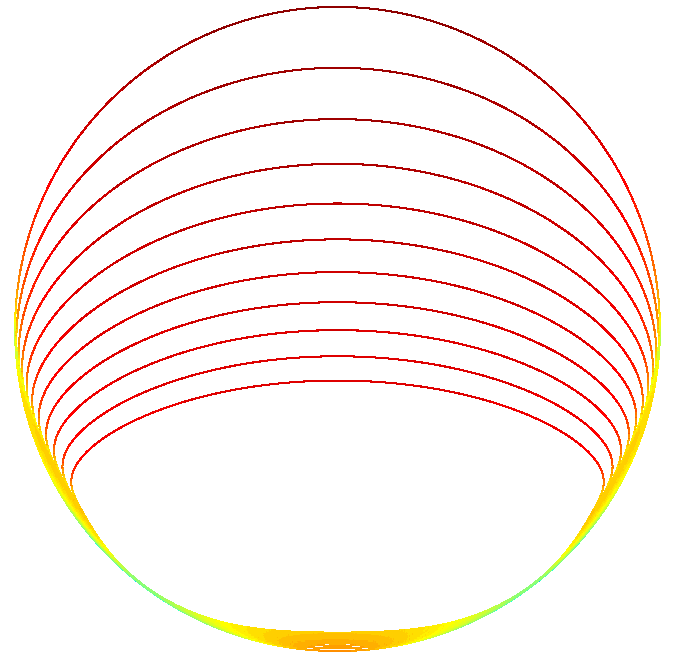
\includegraphics[width = 0.30 \textwidth]{./figs/1b_0d4r1h_shear}
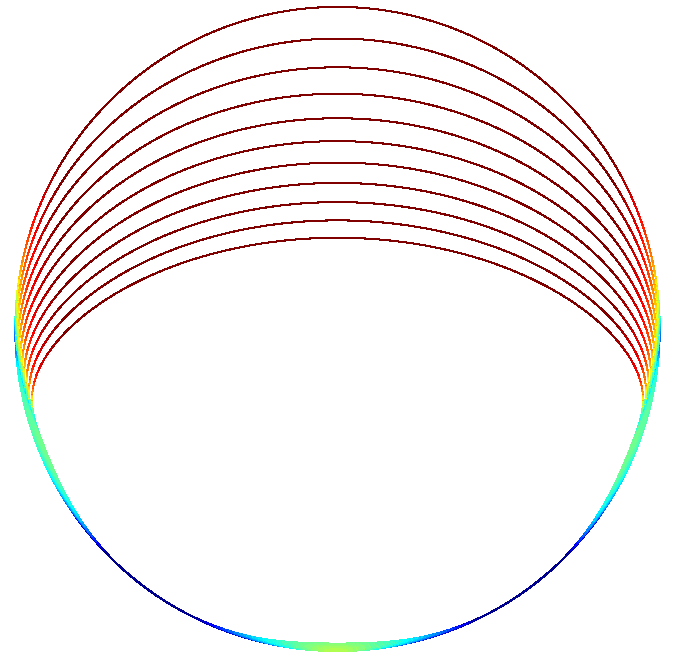
\includegraphics[width = 0.30 \textwidth]{./figs/1b_0d4r0d5h_shear}
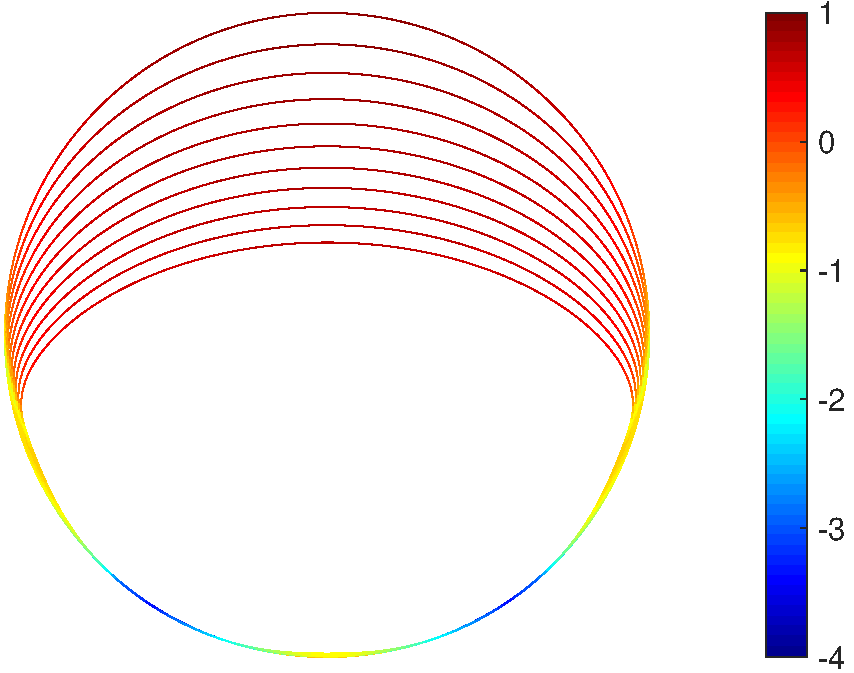
\includegraphics[width = 0.35 \textwidth]{./figs/1b_0d4r0d1h_shear}
\caption{\label{fig:NearWall} 
  A single body eroding in Stokes flow. The color indicates the shear
  stress on the body. Therefore, erosion is fastest in the yellow
  regions and slowest in the blue regions.  In this simulation, we use
  three minimum body-to-wall initial distances $d=h$ (left), $h/2$
  (middle), and $h/10$ (right) with $N_\iin = 256$ discretization points
  on the body, a time step size of $\Dt=10^{-4}$, and smoothing
  parameters $\eps = 15/256$ and $\sigma=10/256$.}
\end{center}
\end{figure}

%%%%%%%%%%%%%%%%%%%%%%%%%%%%%%%%%%%%%%%%%%%%%%%%%%%%%%%%%%%%%%%%%%%%%%%
\subsection{20 nearly touching bodies}
%%%%%%%%%%%%%%%%%%%%%%%%%%%%%%%%%%%%%%%%%%%%%%%%%%%%%%%%%%%%%%%%%%%%%%%
We consider 20 eroding bodies a Hagen-Poiseuille flow.  The background
flow is 
\begin{align}
  \UU(\xx)=U \left[
  \begin{array}{c}
    1-y^2 \\ 0
  \end{array}
  \right].
\end{align}
Initially, $U=1$, and then $U$ is updated at each time step so that the
pressure drop from $x=-2$ to $x=2$ remains constant.  Snapshots of the
bodies at four equispaced times are shown in
Figure~\ref{fig:Eroding20vort}.   The colormap is the vorticity which is
equivalent to the shear stress when restricted to the eroding bodies.
Therefore, erosion is fastest in regions where the magnitude of the
vorticity is largest.

Initially, several of the eroding bodies are close to the outer wall.
In particular, with $h=L_2/N_\out$, the distance between bodies 1, 6,
13, and 15 are $1.3h$, $2.9h$, $2.8h$, and $1.3h$, respectively.  In
addition, since each body is discretized with $N_\iin=256$ points, the
distance between several pairs of eroding bodies is too small to be
accurately resolved at the prescribed resolution.  Particular pairs
include bodies 1 \& 6, 3 \& 9, 6 \& 8, and 14 \& 18.  By using the
Barycentric quadrature rule, the interaction between these
nearly-touching bodies can be accurately resolved at the prescribed
resolution.

In~\cite{qua-moo2018}, we observed that erosion causes the space
between nearly touching bodies to quickly expand, and flat faces develop
along the region of near contact.  This qualitative behavior is also
observed In Figure~\ref{fig:Eroding20vort}, such as between bodies 3
\&4 and 15 \& 16.  However, by resolving bodies that are
much closer to one another when compared to our previous
work~\cite{qua-moo2018}, we see that it is possible for very little
erosion to occur between a pair of bodies.  In particular, for pairs of
bodies where the channel between the bodies is nearly perpendicular to
the main flow direction (bodies 1 \& 6, 3 \& 9, and 13 \& 15), there is
very little shear stress and the effect of erosion is slight. 

\begin{figure}[H]
\begin{center}
  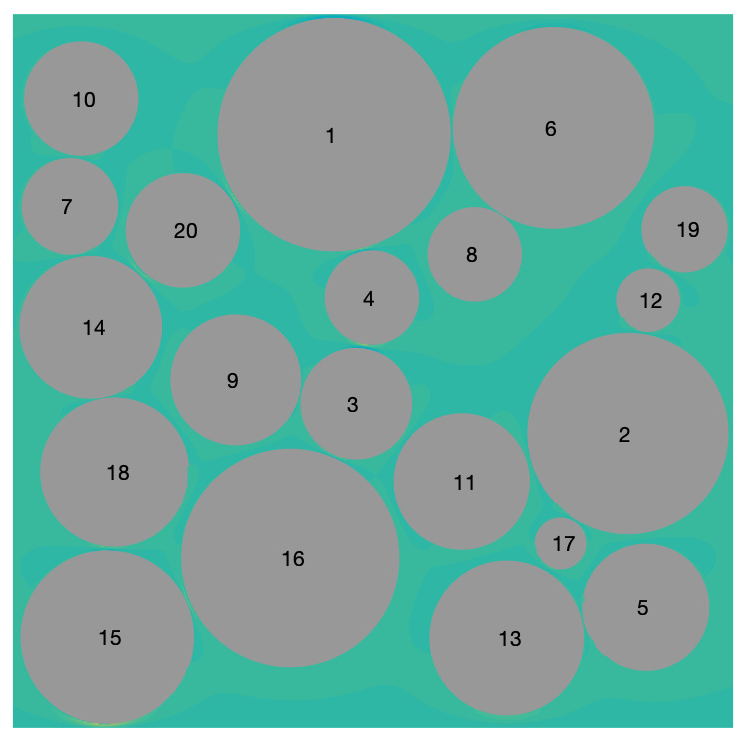
\includegraphics[height=0.43\textwidth]{./figs/20b_dense1}
  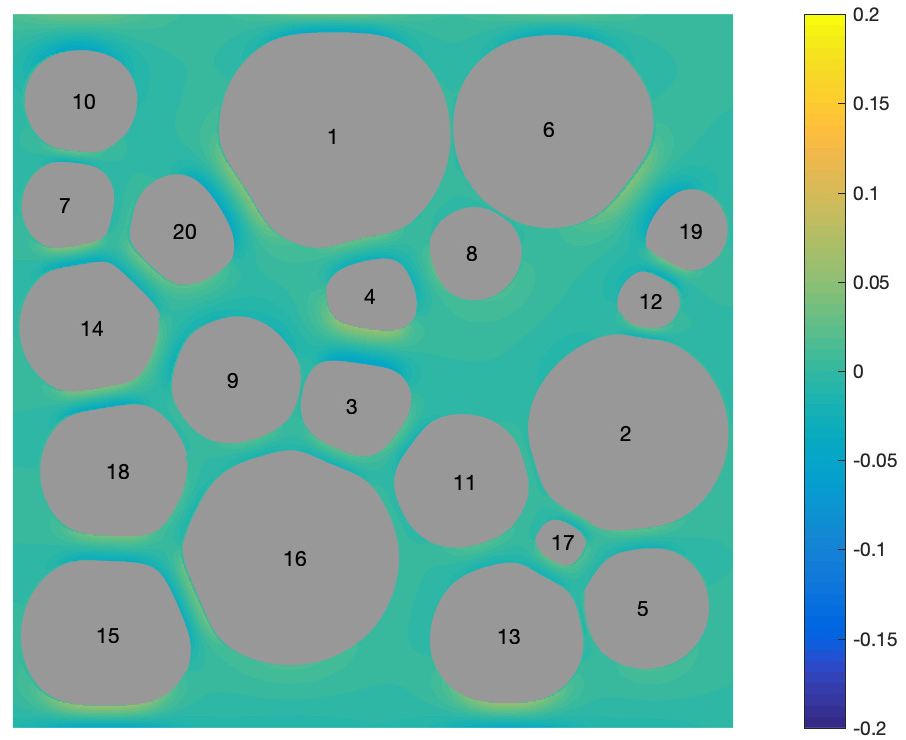
\includegraphics[height=0.43\textwidth]{./figs/20b_dense101} \\
  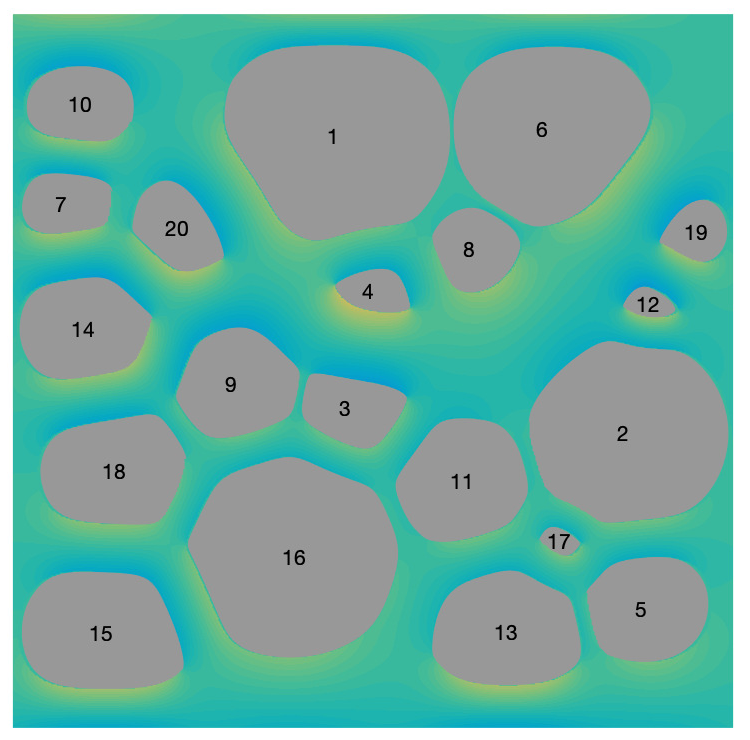
\includegraphics[height=0.43\textwidth]{./figs/20b_dense201}
  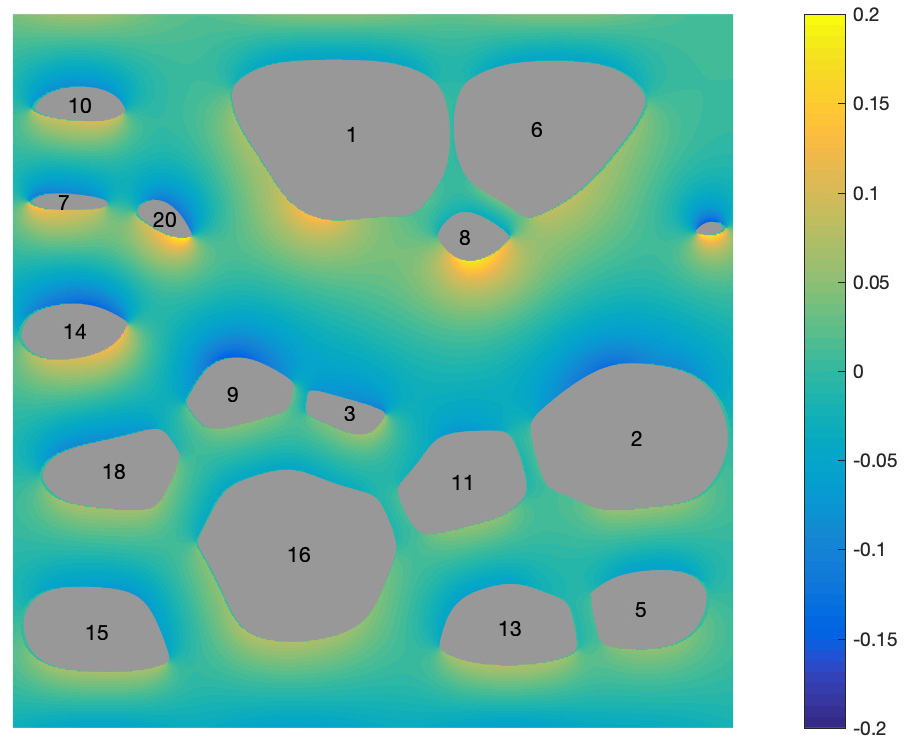
\includegraphics[height=0.43\textwidth]{./figs/20b_dense301}
%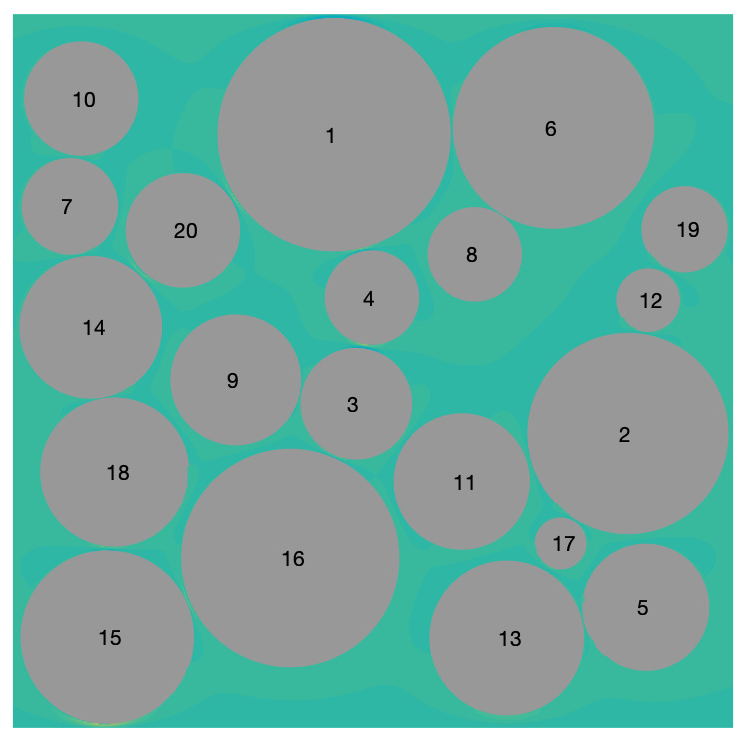
\includegraphics[width = 0.42 \textwidth]{./figs/20b_dense1}
%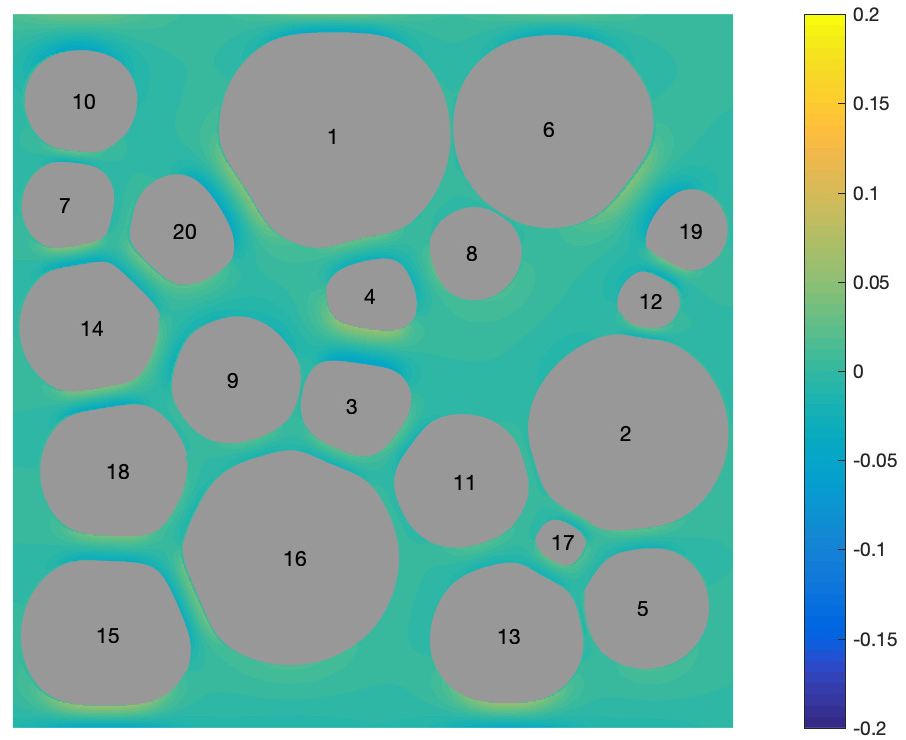
\includegraphics[width = 0.507 \textwidth]{./figs/20b_dense101}\\
%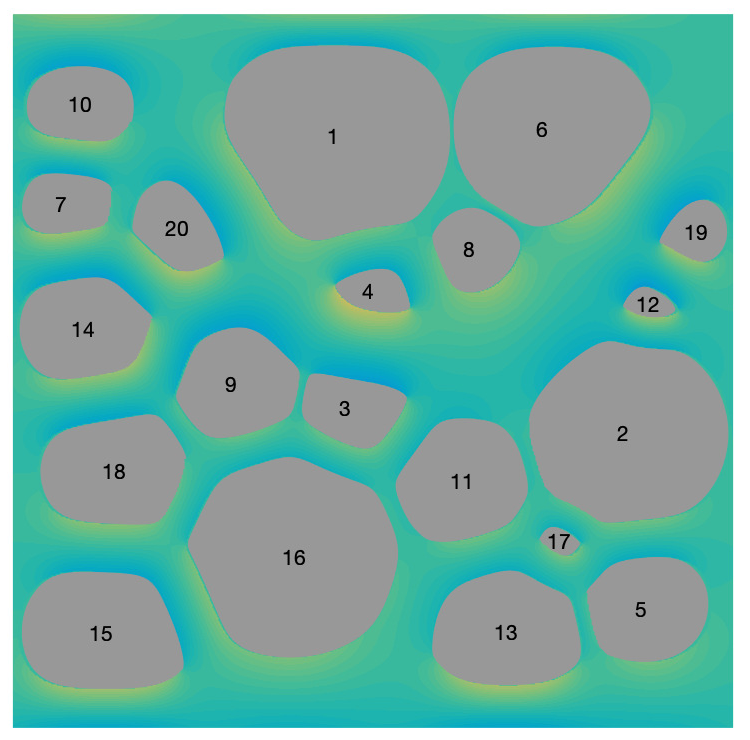
\includegraphics[width = 0.42 \textwidth]{./figs/20b_dense201}
%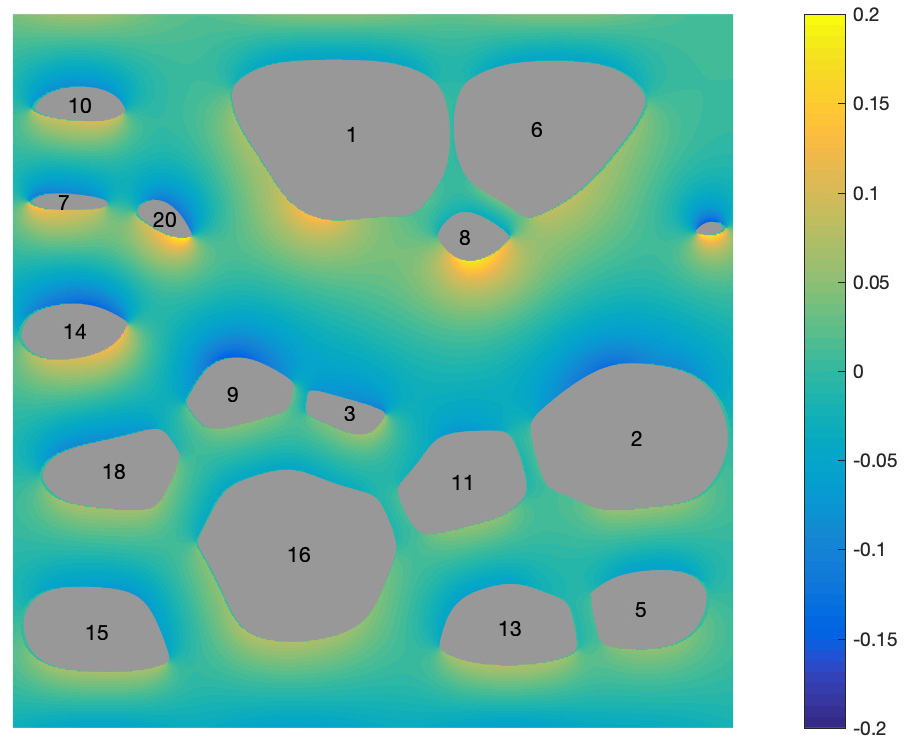
\includegraphics[width = 0.507 \textwidth]{./figs/20b_dense301}
\caption{\label{fig:Eroding20vort} Erosion of 20 nearly touching bodies
  with the fixed pressure drop condition. The color is the vorticity of
  the fluid. The 4 snapshots are evenly spaced in time. We use $N_\iin =
  256$ discretization points on the body, a time-step of $\Dt=10^{-4}$,
  and smoothing parameters of $\eps= 15/256$ and $\sigma=10/256 $. In
  the forth frame, bodies 4, 12, and 17 have vanished completely, and
  body 19 has almost completely eroded.}
\end{center}
\end{figure}

In this example, we also observe that erosion creates a network of
channels from the inlet to outlet where the velocity and vorticity, and
therefore erosion rate, are much larger than the other regions.  These
channels can be further visualized by considering the streamlines at
several configurations of the eroding body.  In
Figure~\ref{fig:Eroding20tracer}, we simulate 200 tracers that are
initially to the left of the porous region and equispaced in $y$.  There
are two clear region where the tracers pass through the geometry
much faster than the other regions.  To illustrate the ability of the
Barycentric quadrature formula, streamlines very close to the eroding
bodies are illustrated in Figure~\ref{fig:Eroding20zoom}. 

\begin{figure}[H]
\begin{center}
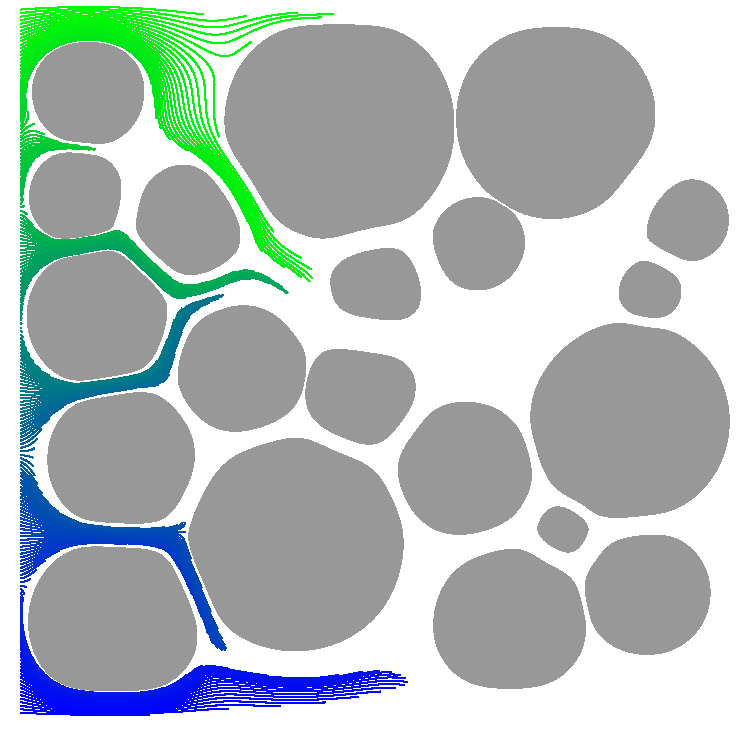
\includegraphics[width = 0.32 \textwidth]{./figs/tracer_20b30}
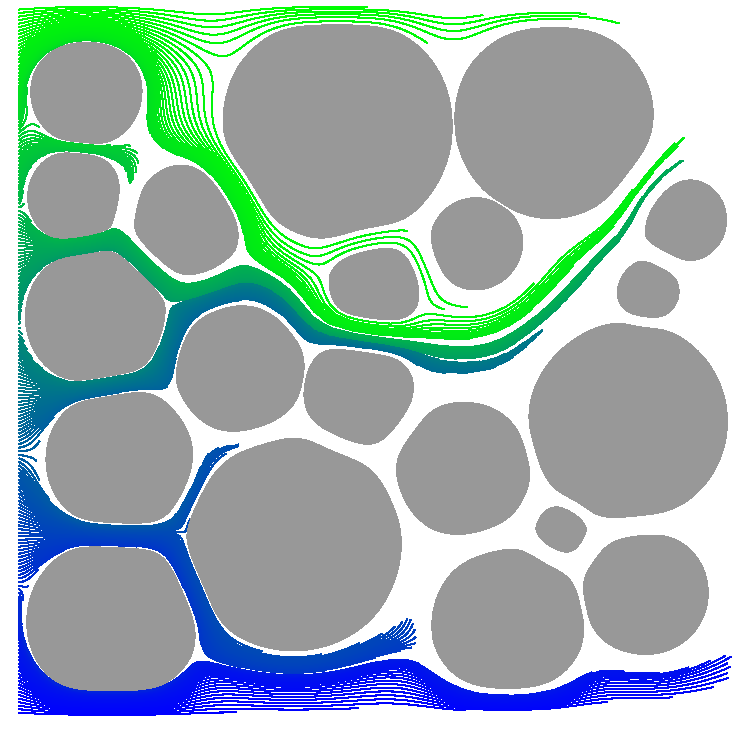
\includegraphics[width = 0.32 \textwidth]{./figs/tracer_20b60}
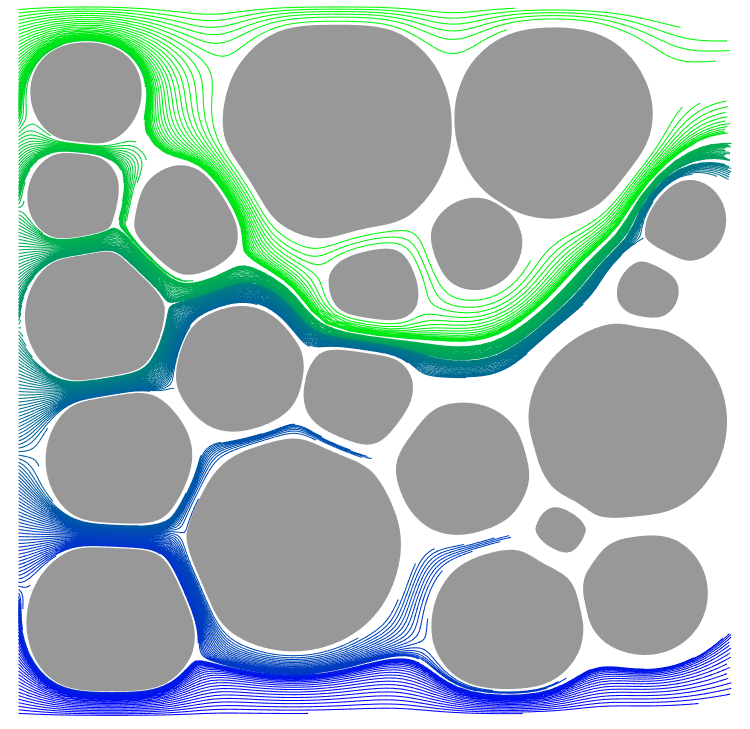
\includegraphics[width = 0.32 \textwidth]{./figs/tracer_20b90}\\

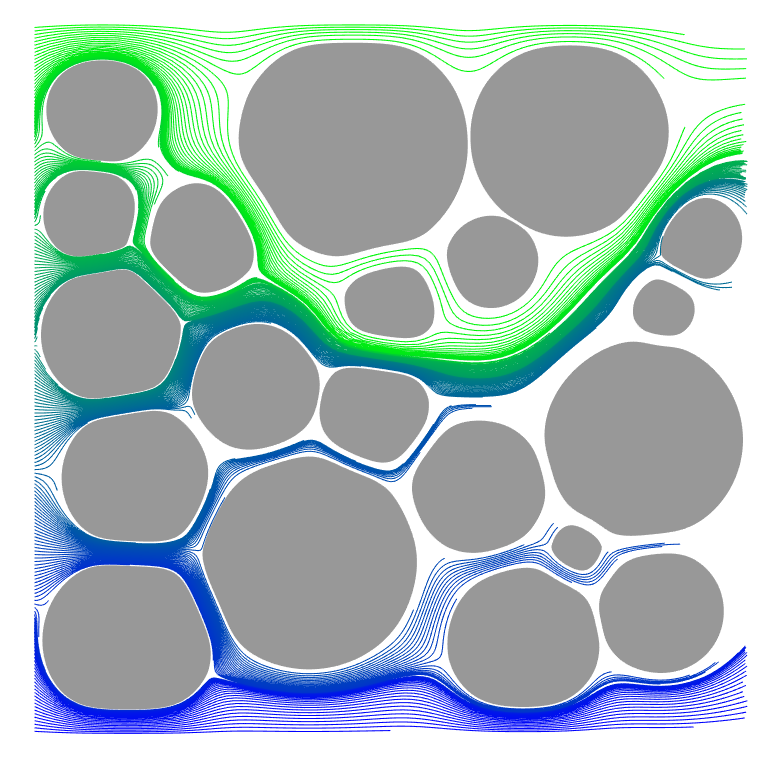
\includegraphics[width = 0.32 \textwidth]{./figs/tracer_20b120}
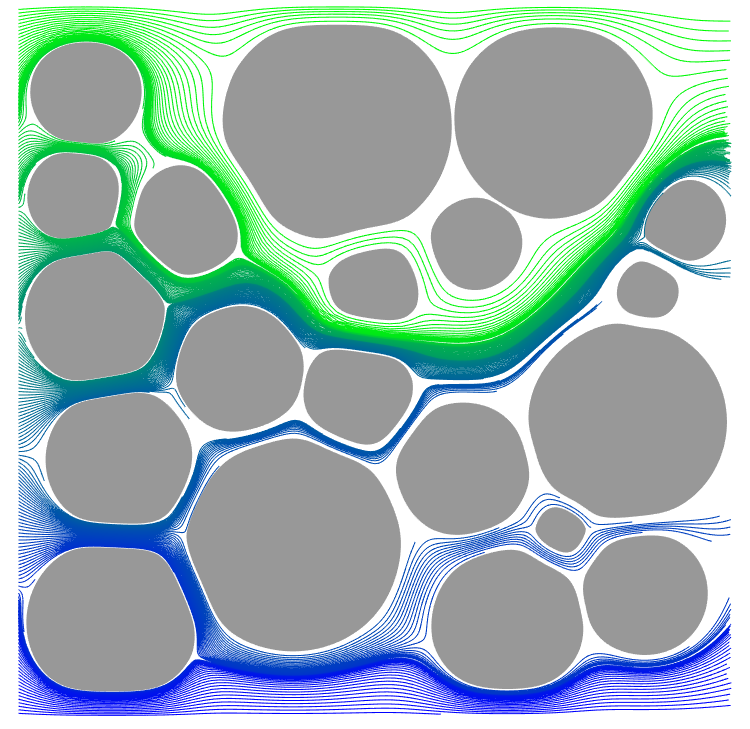
\includegraphics[width = 0.32 \textwidth]{./figs/tracer_20b150}
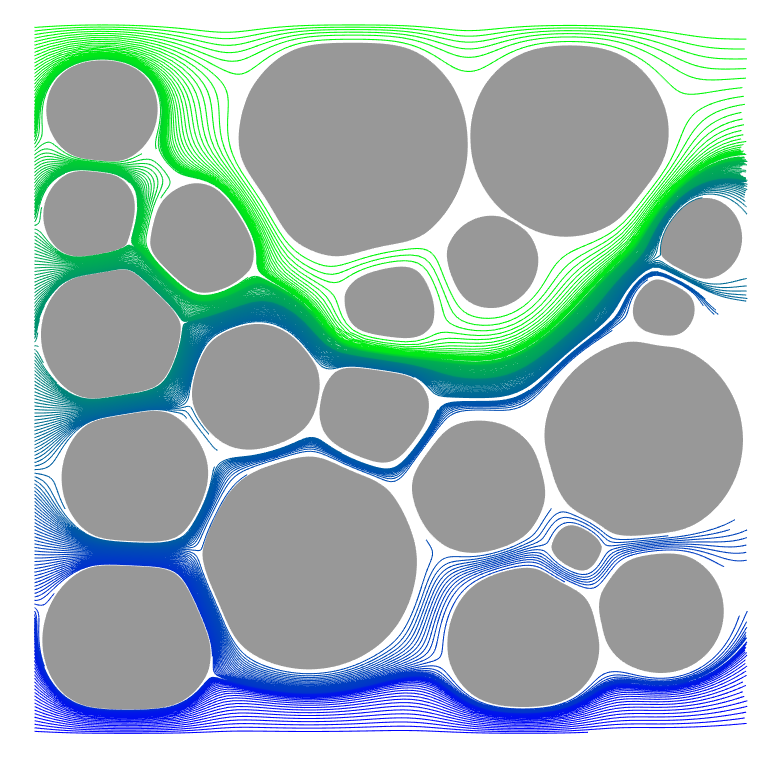
\includegraphics[width = 0.32 \textwidth]{./figs/tracer_20b180}\\

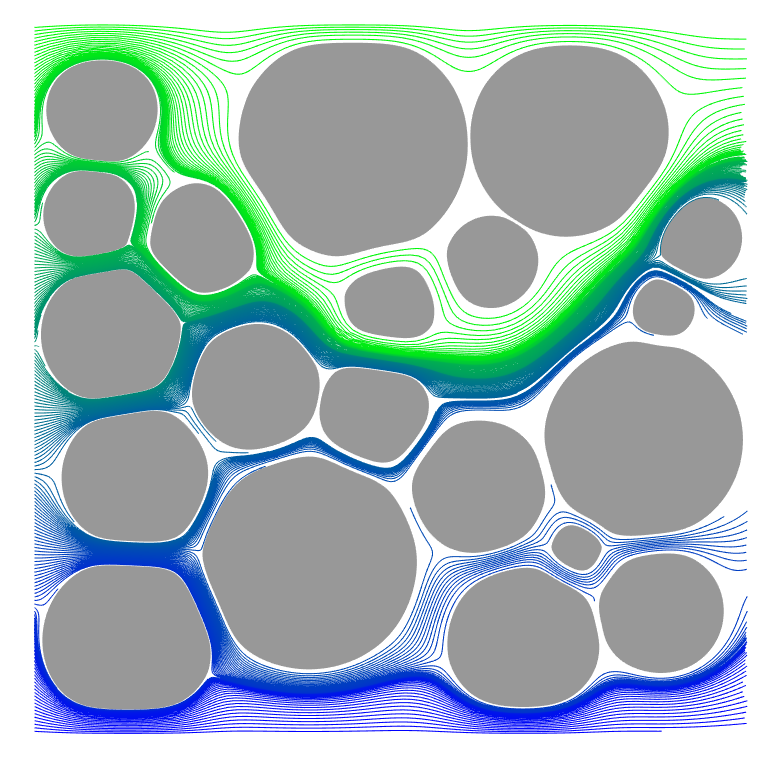
\includegraphics[width = 0.32 \textwidth]{./figs/tracer_20b210}
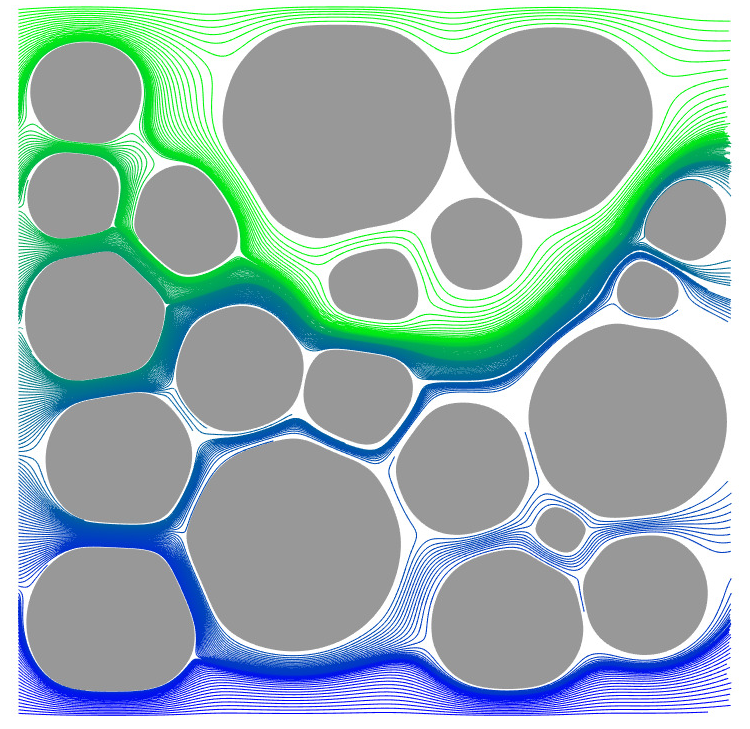
\includegraphics[width = 0.32 \textwidth]{./figs/tracer_20b240}
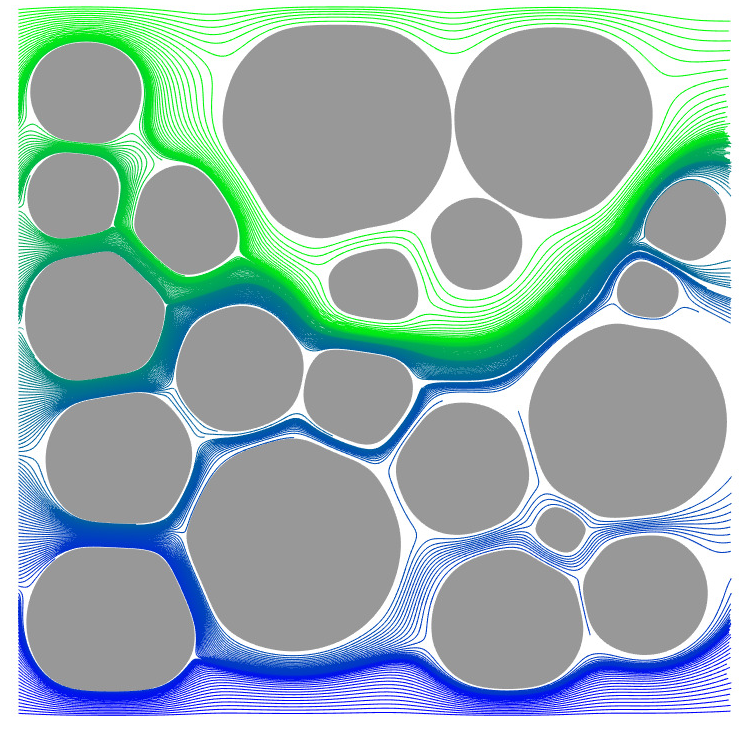
\includegraphics[width = 0.32 \textwidth]{./figs/tracer_20b270}
\caption{\label{fig:Eroding20tracer}The trajectories of 200 tracers in
  the fluid with 20 bodies. The 9 snapshots are evenly spaced in time.
  The tracers are evenly spread in the $y$-direction and released at
  $x=-1$.}
\end{center}
\end{figure}

\begin{figure}[H]
\begin{center}
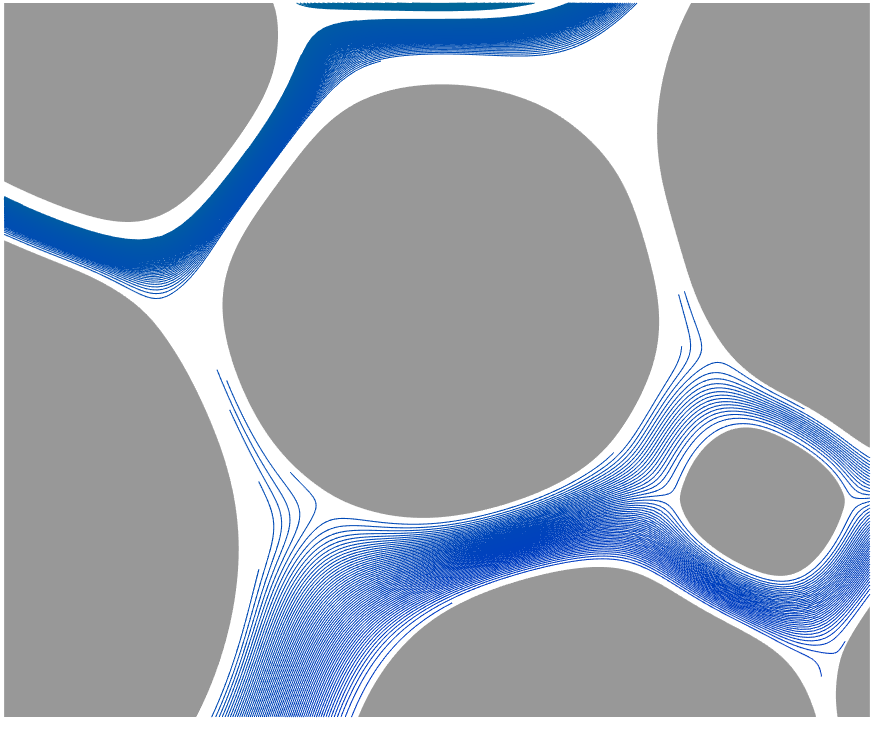
\includegraphics[width = 0.32\textwidth]{./figs/tracer_20b210_zoom}
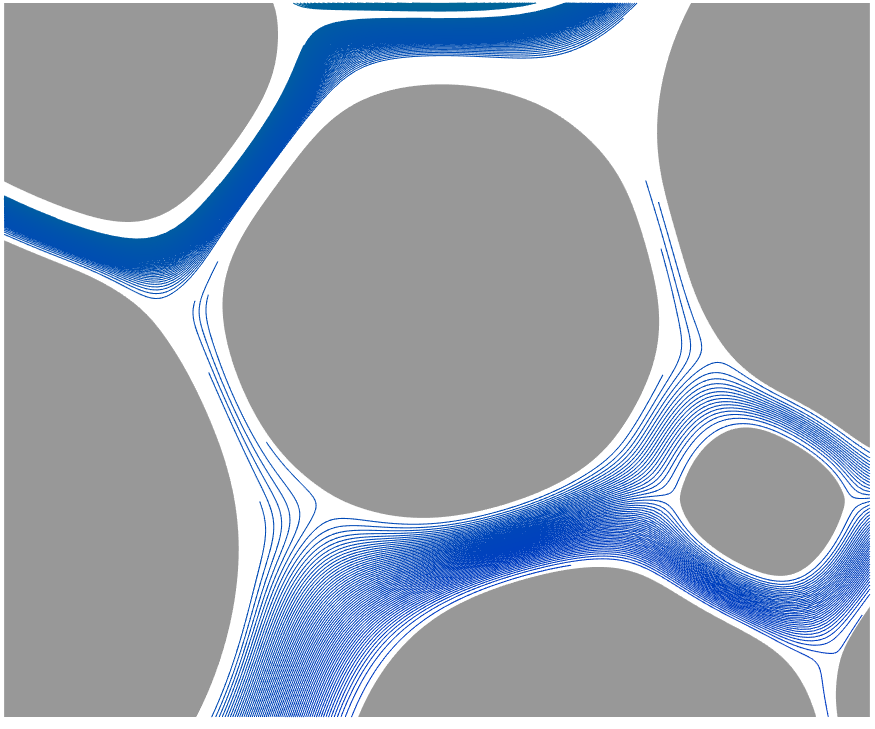
\includegraphics[width = 0.32\textwidth]{./figs/tracer_20b240_zoom}
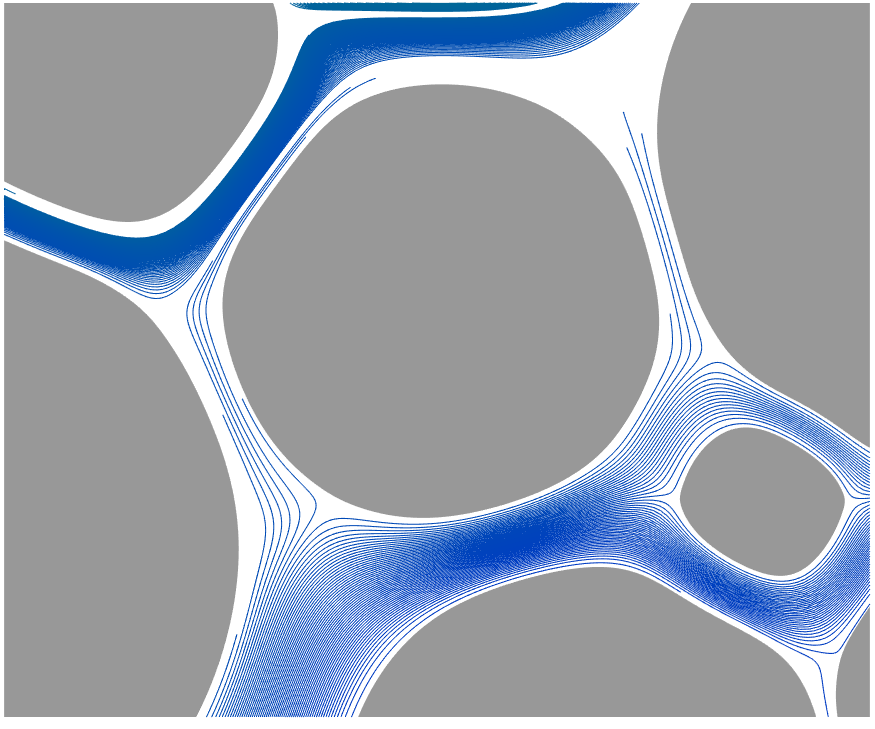
\includegraphics[width = 0.32\textwidth]{./figs/tracer_20b270_zoom}
\caption{\label{fig:Eroding20zoom}The zoom windows in the last three
  frames of Figure~\ref{fig:Eroding20tracer}. The trajectories of
  tracers around the bodies. Since we use a Barycentric quadrature rule
  and the fourth order Runge Kutta method, the tracers can be very close
  to but not penetrate the bodies.}
\end{center}
\end{figure}



{\color{red} 
Besides the channels between two bodies, there is a single channel goes
across the domain horizontally and the flow has been concentrated in
this channel.  In the second frame of Fig.~\ref{fig:Eroding20vort}, this
channel is between bodies 1 \& 20, 1 \& 9, 4 \& 3, 8 \& 11, 8 \& 2, 6 \&
12, and 6 \& 19.  We can get a better understanding of this channel from
the trajectories of tracers in Fig.~\ref{fig:Eroding20tracer}.  In the
top three frames of  Fig.~\ref{fig:Eroding20tracer}, the flow (or
tracer) first comes from three small channels between outer wall \& body
10, bodies 7 \& 14, and bodies 14 \& 18, then the three branches become
one and go into the main channel between bodies 1 \& 9.  From the first
frame to the forth frame of Fig.~\ref{fig:Eroding20vort}, this channel
is expanding faster than other channel and bodies 4 \& 12 has vanished
and body 19 is almost gone in the forth frame.  The reason of fast
expansion of this channel is the high vorticity.  In the forth frame of
Fig.~\ref{fig:Eroding20vort}, we could see the vorticity is relatively
high on the side of bodies which form this channel so the bodies are
eroded fast on the side of this channel or have vanished completely.

Furthermore, how long the body lasts for depends on not only the size of
the body but also the location of the body.  For example, the first
three vanishing bodies are body 12 (as t=0.0256), 4 (as t=0.0278), then
17 (as t=0.0287).  Since body 4 is located in the main flow channel so
the body 4 is vanished earlier than body 17 although the initial size of
body 4 is larger than the size of body 17.  This channel will keep
expanding and the bodies around this channel will vanish earlier than
others.  After body 17, the next 8 vanished bodies with respect to time
are body 19 (as t=0.0312),  body 7 (as t=0.0325), body 20 (as t=0.0329),
body 8 (as t=0.0349), body 10 (as t=0.0353), body 3 (as t=0.0356), body
14 (as t=0.0363), then body 9 (as t=0.0376).  All of these eight bodies
were around this channel before they are gone.

For the flat faces at the sites of near contact, since we put the body
be close to one another so we are able to see all the channels between
two close bodies have flat faces.  Besides the channels between bodies,
we also observe the flat faces on the bodies which are close to the
outer wall. For example, we see the flat faces on the top of bodies 1 \&
6 and the bottom of bodies 13 \& 15.  

Since we use a Barycentric quadrature rule to approximate the velocity
of tracers and apply the fourth order Runge Kutta method to find the new
locations of tracers in each step, the tracers can be very close to but
not penetrate the bodies.  Those body-closed tracers are moving
perfectly so we are able to observe the details of the interaction of
bodies and fluid.  Although the direction of flow is from left to right,
the tracers will not only travel horizontally but also vertically.  In
the last three frames of Fig.~\ref{fig:Eroding20tracer}, some tracers
climb up from right to left around the body.  There are zoom windows of
the climbing tracers trajectories in Fig.~\ref{fig:Eroding20zoom} and
they are taken from the last three frames of
Fig.~\ref{fig:Eroding20tracer} with more tracers.  In
Fig.~\ref{fig:Eroding20zoom} the tracers around the center body first go
from the channel below the body, climb up to the left, then go to the
right and join another tracers in the channel above the body. 

In Fig.~\ref{fig:Eroding20area} we
measure the area occupied by bodies 
during the eroding. In the beginning, 62.32\% of area of $[-1,1] \times
[-1,1]$ is occupied by 20 bodies. Then the eroding speed is increasing
when more and more bodies are vanished in the fluid and 
the maximum eroding speed happens when 7.57\% of area of $[-1,1] \times
[-1,1]$ is occupied by 8 bodies. After that the speed drops rapidly to 0 when
all the bodies are vanished completely.

Fig.~\ref{fig:Eroding20flowrate} we record the flow rate $U$ quantifily
during the eroding. Since we simulate the erosion by applying fixed pressure drop 
the flow rate $U$ is small when there are many bodies in the fluid and 
when the area occupied by bodies is getting smaller $U$ is getting larger.
When all the bodies have vanished completely the flow rate $U$ is equal to 1.
In Fig.~\ref{fig:Eroding20flowrate}, the flow rate increases exponentially 
with growth rate close to $\ln10^4$. 


In Fig.~\ref{fig:Eroding20tort} we use tortuosity to analysis the effect
of the geometrical structure on fluid velocity field. In
Fig.~\ref{fig:Eroding20tort}(a) the graph represents the ratio of the
x-component velocity u(-1, y) to its maximum velocity $u_{max}=6.2281
\times 10^{-4}$ at equal spreading tracers on the cross section (x=-1
and y in [-1,1]). The velocity is continuous along the cross section and
acting as several Poiseuille flows. This velocity graph is different
from the one in~\cite{matyka2008tortuosity} since we choose our cross
section to be the beginning of the flow before the fluid touches any
body. In Fig.~\ref{fig:Eroding20tort}(b) we record the local tortuousity
$\tau$ of the tracers at the cross section. This graph is not continuous
and the jumps in $\tau$ mean that the initial neighbor tracers have been
seperated by the bodies. 

In Fig.~\ref{fig:Eroding20tort}(c) we calculate the difference of $\tau$ at two neighboring tracers 
and draw 
In Fig.~\ref{fig:Eroding20tort}(d) 
}


\begin{figure}[H]
\begin{subfigure}[b]{0.5\textwidth}
\includegraphics*[width =\linewidth]{./figs/porosity20dense}
\caption{}
\end{subfigure}%
\begin{subfigure}[b]{0.5\textwidth}
\includegraphics*[width =\linewidth]{./figs/erodingspeed20dense}
\caption{}
\end{subfigure}
\caption{\label{fig:Eroding20area}  The area fraction of 20 nearly
  touching eroding bodies and the eroding speed verse time.}
\end{figure}


\begin{figure}[H]
%\begin{subfigure}[b]{0.5\textwidth}
\center
\includegraphics*[width =0.5\linewidth]{./figs/flow_rate20dense}
%\caption{}
%\end{subfigure}%
%\begin{subfigure}[b]{0.5\textwidth}
%\includegraphics*[width =\linewidth]{./figs/flow_rate20dense}
%\caption{}
%\end{subfigure}
\caption{\label{fig:Eroding20flowrate}  The incoming flow rate of U verse time.}
\end{figure}

\begin{figure}[H]
\begin{subfigure}[b]{0.5\textwidth}
\includegraphics*[width =\linewidth]{./figs/velocity_loc}
\caption{}
\end{subfigure}%
\begin{subfigure}[b]{0.5\textwidth}
\includegraphics*[width =\linewidth]{./figs/tort_local}
\caption{}
\end{subfigure}
\begin{subfigure}[b]{0.5\textwidth}
\includegraphics*[width =\linewidth]{./figs/diff_tort}
\caption{}
\end{subfigure}%
\begin{subfigure}[b]{0.5\textwidth}
\includegraphics*[width =\linewidth]{./figs/uminDumax}
\caption{}
\end{subfigure}
\caption{\label{fig:Eroding20tort} The tortuosity of the 20 nearly touching bodies}
\end{figure}

\begin{figure}[H]
\center
\includegraphics*[width =0.5\linewidth]{./figs/tort_diff_top20}
\caption{\label{fig:Eroding20tort_traj} The largest 20 difference of the length of 
two neighbor tracers' trajectories in
 20 nearly touching bodies eroding}
\end{figure}


%%%%%%%%%%%%%%%%%%%%%%%%%%%%%%%%%%%%%%%%%%%%%%%%%%%%%%%%%%%%%%%%%%%%%%%
\subsection{50 nearly touching bodies}
%%%%%%%%%%%%%%%%%%%%%%%%%%%%%%%%%%%%%%%%%%%%%%%%%%%%%%%%%%%%%%%%%%%%%%%
{\color{red}
The second nearly touching bodies case is 50 bodies in a Hagen-Poiseuille flow.
}

%%%%%%%%%%%%%%%%%%%%%%%%%%%%%%%%%%%%%%%%%%%%%%%%%%%%%%%%%%%%%%%%%%%%%%%
\subsection{100 bodies}
%%%%%%%%%%%%%%%%%%%%%%%%%%%%%%%%%%%%%%%%%%%%%%%%%%%%%%%%%%%%%%%%%%%%%%%
{\color{red}
This case is 100 bodies in a Hagen-Poiseuille flow.
}
\begin{figure}[H]
\begin{center}
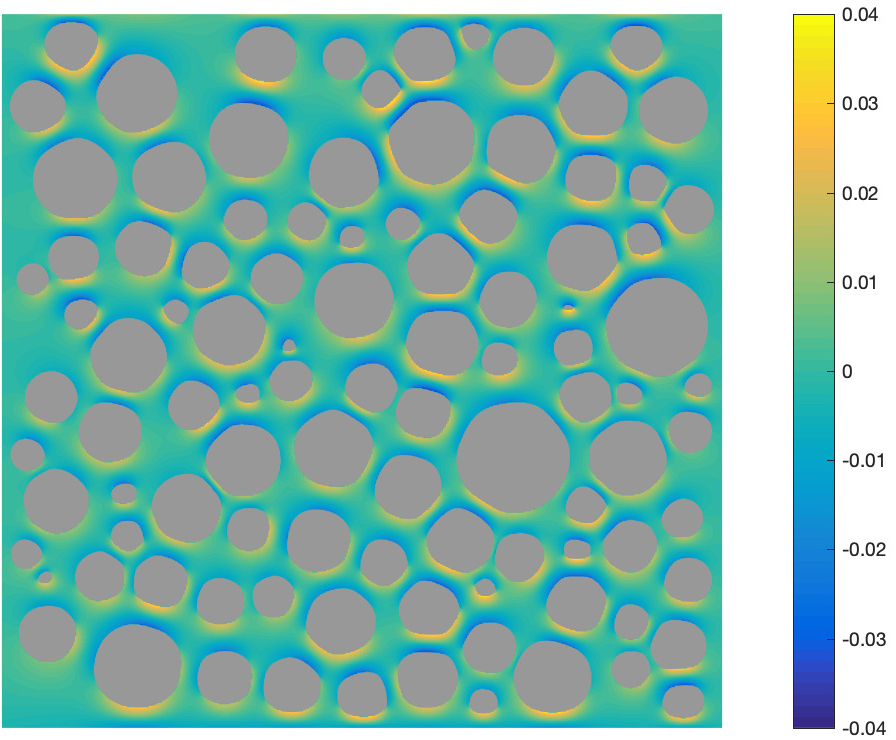
\includegraphics[width = 0.8\textwidth]{./figs/100b_50}
\caption{\label{fig:Eroding100vort} Erosion of 100 bodies with the
  fixed-pressure-drop condition. The color is the vorticity of fluid. In
  this simulation, we use $N_\iin = 256$ discretization points on the
  body, $N_\out = 1024$ points on the outer wall, a time-step of
  $\Dt=10^{-4}$, and smoothing parameters of $\eps= 15/256$ and
  $\sigma=10/256 $}
\end{center}
\end{figure}
\begin{figure}[H]
\begin{center}
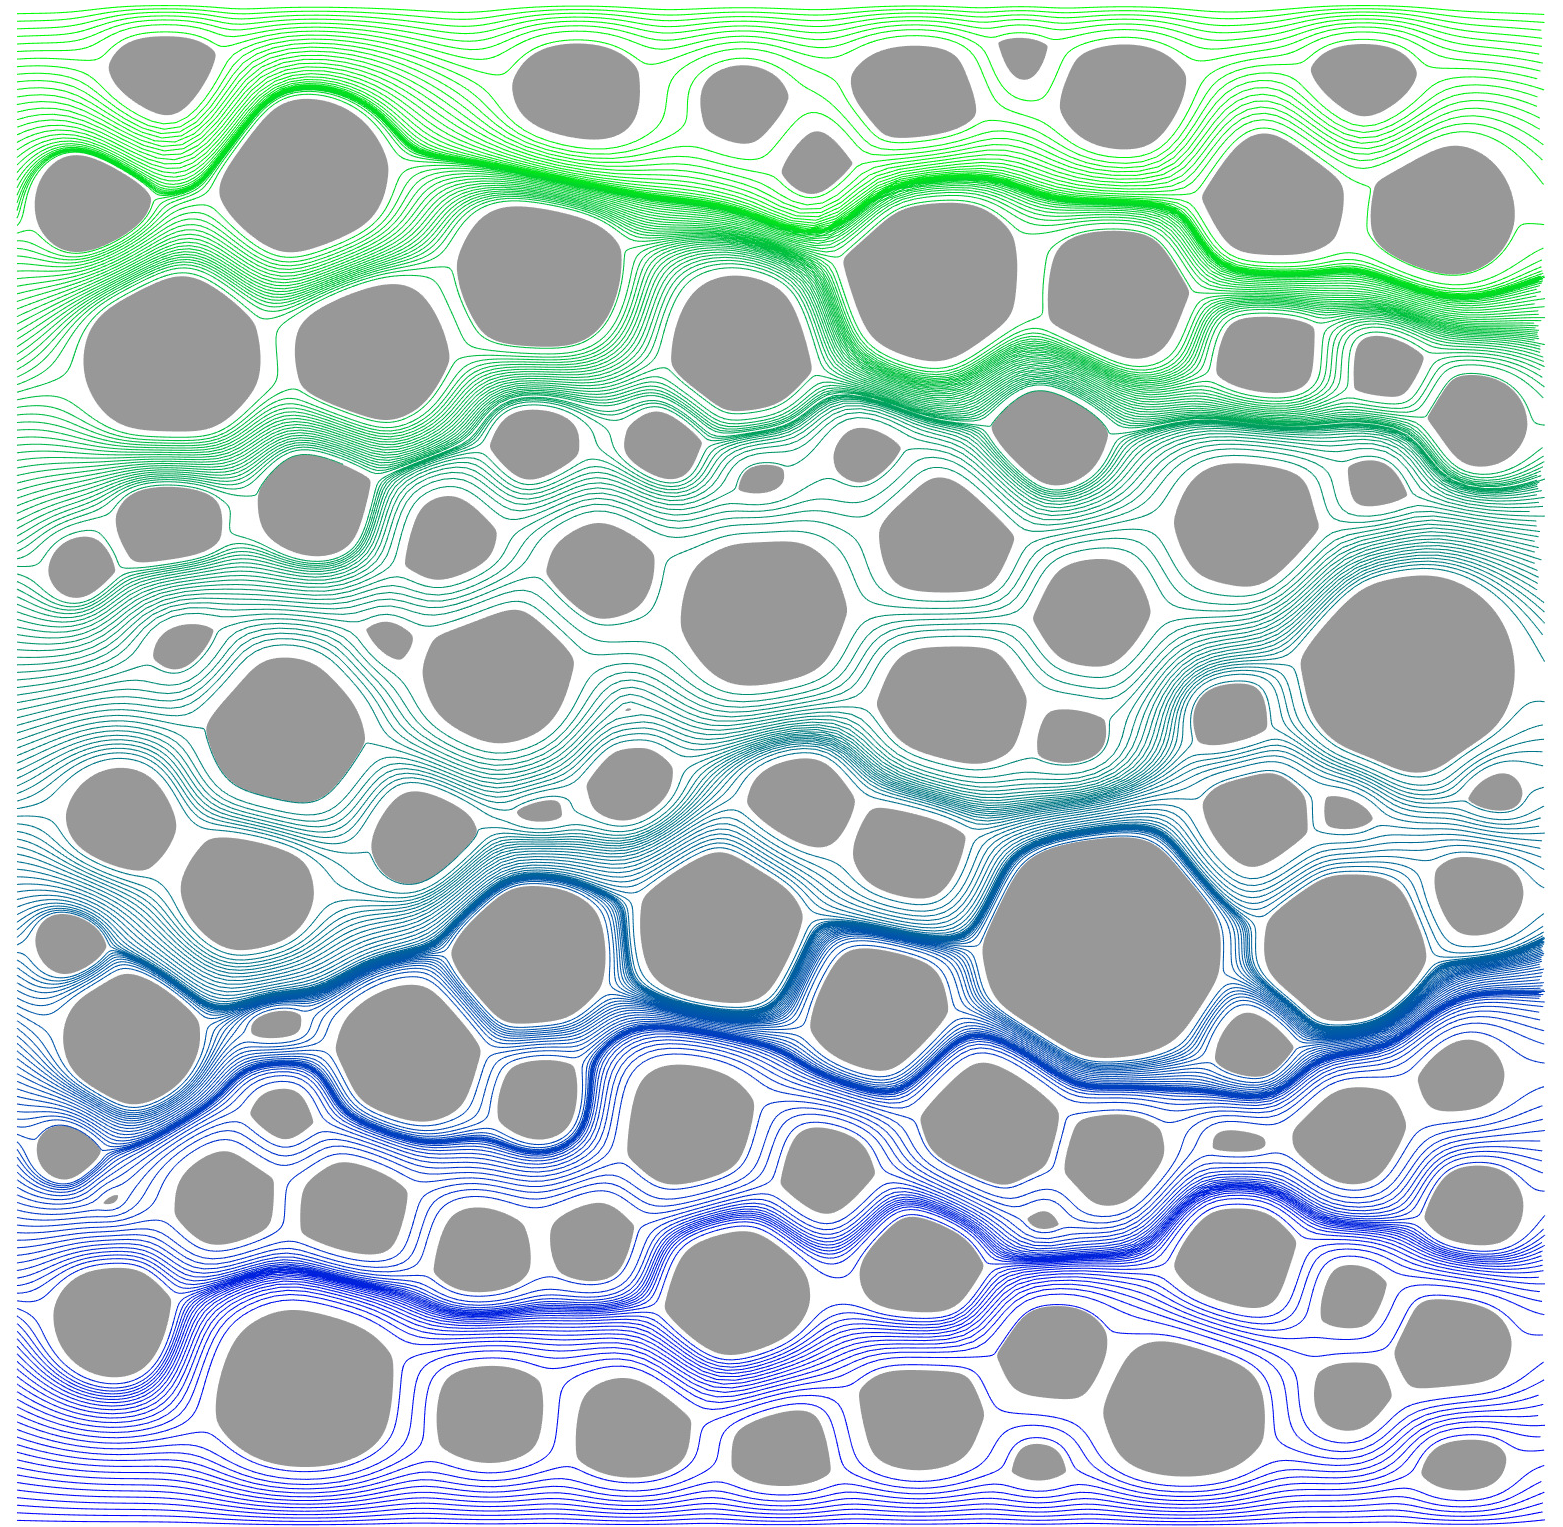
\includegraphics[width = 0.8\textwidth]{./figs/100b_t100tracer}
\caption{\label{fig:Eroding100tracer} The trajectories of 200 tracers in the fluid with 100 bodies}
\end{center}
\end{figure}


%%%%%%%%%%%%%%%%%%%%%%%%%%%%%%%%%%%%%%%%%%%%%%%%%%%%%%%%%%%%%%%%%%%%%%%
\section{Conclusions}
\label{s:conclusions}
%%%%%%%%%%%%%%%%%%%%%%%%%%%%%%%%%%%%%%%%%%%%%%%%%%%%%%%%%%%%%%%%%%%%%%%


%%%%%%%%%%%%%%%%%%%%%%%%%%%%%%%%%%%%%%%%%%%%%%%%%%%%%%%%%%%%%%%%%%%%%%%
\paragraph{\bf Acknowledgments} BQ and NM were supported by Florida
State University startup funds and Simons Foundation Mathematics and
Physical Sciences-Collaboration Grants for Mathematicians.

\bibliographystyle{plainnat} 
\biboptions{sort&compress}
\bibliography{refs}


\end{document}








%old stuff%
%%%%%%%%%%%%%%%%%%%%%%%%%%%%%%%%%%%%%%%%%%%%%%%%%%%%%%%%%%%%%%%%%%%%%%%%
%\subsection{boundary integral equation formulation} 
%\label{sec:bies}
%add an introduction why we do not use the double-layer potentials of stokes equations but the double-layer potentials of laplace equations to solve stokes equation when we use barycentric approach (or complex variable approach).
%
%\subsubsection{laplace's equations from $\rdb^2$ to $\cdb$ }
%
%let $\omega$ be the domain of fluid. the boundary of $\omega$ is $\gamma$ and the outward normal vector on $\gamma$ is ${\bf n_y}=(n_1,n_2)$.
%
%consider a laplace's equations with dirichlet boundary condition
%\begin{equation}\label{laplace}
%  \begin{cases}
%    \delta {\bf u}=0, & \text{in}\,\,\, \omega \in \rdb^2;\\
%    {\bf u}={\bf f}, & \text{on}\,\,\, \gamma.
%  \end{cases}
%\end{equation}
%
%Let ${\bf x}=(x_1,x_2), {\bf y}=(y_1,y_2)$. Then we have ${\bf r}={\bf x} - {\bf y}$ and $\rho=|\bf r|$.
%The double-layer potential which solves \eqref{Laplace} is 
%\begin{align*}
%\D[\sigma]({\bf x})&=\frac{1}{2\pi}\displaystyle\int_{\Gamma} \frac{{\bf r} \cdot {\bf n_y}}{\rho^2}\sigma({\bf y})ds_y,
%%\frac{1}{2\pi}\displaystyle\int_{\Gamma}\frac{\partial}{\partial {\bf n_y}} \log |{\bf x}-{\bf y}| \sigma({\bf y})ds_y,\\ \\
%%&=\frac{-1}{2\pi}\int_{\Gamma}\frac{{\bf r}\cdot{\bf n_y}}{\rho^2} \sigma({\bf y})ds_y\\ \\
%%&=\frac{-1}{2\pi}\int_{\Gamma}\frac{n_1(x_1-y_1)+n_2(x_2-y_2)}{(x_1-y_1)^2+(x_2-y_2)^2} \sigma({\bf y})ds_y 
%\numberthis\label{DLP:real}
%\end{align*}
%where $\sigma$ is the density function on the boundary $\Gamma$.
%
%
%Consider a Cauchy integral 
%\begin{equation}\label{CI}
%v({x})=\frac{1}{2\pi i}\int_{\Gamma}\frac{\sigma({ y})}{{ y}-{ x}} d{ y},\,\,\,\,\,\,\,\,\, \forall { x} \in \Cdb\setminus \Gamma.
%\end{equation}
%where ${ x}=x_1+ix_2$, $ { y}=y_1+iy_2$, ${ n_y}=n_1+i n_2$ and $d{ y}=i {n_y}ds_y$. It can be shown that 
%the real part of the Cauchy integral in \eqref{CI} is equivalent to the double-layer potential in \eqref{DLP:real}. 
%
%
%\subsubsection{From Stokes DLP to Laplace DLPs}
%
%Let ${\bf x}=(x_1,x_2), {\bf y}=(y_1,y_2)$. Then we have ${\bf r}={\bf x} - {\bf y}$ and $\rho=|\bf r|$.
%
%
%The Stokes double-layer potential  is
%\begin{equation}\label{StokesDLP1}
%\D[\boldsymbol\sigma]({\bf x}):=\frac{1}{\pi}\int_{\Gamma}\left(\frac{{\bf r} \cdot {\bf n_y}}{\rho^2}\frac{{\bf r} \otimes {\bf r}}{\rho^2}\right) {\boldsymbol\sigma({\bf y})} d s_y.
%\end{equation}
%We could rewrite the Stokes DLP in terms of the Laplace DLP as
%\begin{align*}\label{StokesDLP2}
%\D[\boldsymbol\sigma]({\bf x})=\frac{1}{2\pi}\int_{\Gamma}&\frac{{\bf n_y}}{\rho^2}({\bf r} \cdot {\boldsymbol \sigma})ds_y+\frac{1}{2\pi}\nabla\int_{\Gamma}\frac{{\bf r} \cdot {\bf n_y}}{\rho^2}({\bf y} \cdot{\boldsymbol \sigma})ds_y\\
%&-\frac{1}{2\pi}x_1 \nabla\int_{\Gamma}\frac{{\bf r} \cdot {\bf n_y}}{\rho^2}\sigma_1ds_y-\frac{1}{2\pi}x_2\nabla\int_{\Gamma}\frac{{\bf r} \cdot {\bf n_y}}{\rho^2}\sigma_2ds_y. \numberthis
%\end{align*}
%

 
%%%%%%%%%%%%%%%%%%%%%%%%%%%%%%%%%%%%%%%%%%%%%%%%%%%%%%%%%%%%%%%%%%%%%%%%
%\subsection{Computing the shear stress}
%\label{sec:shearStressLP}
%
%To calculate the shear stress, we need to know the gradient of double-layer potential in \eqref{StokesDLP2} 
%\begin{align*}\label{SSLP}
%\nabla\D[\boldsymbol\sigma]({\bf x})=\frac{1}{2\pi}\nabla\int_{\Gamma}&\frac{{\bf n_y}}{\rho^2}({\bf r} \cdot {\boldsymbol \sigma})ds_y+\frac{1}{2\pi}\nabla^2\int_{\Gamma}\frac{{\bf r} \cdot {\bf n_y}}{\rho^2}({\bf y} \cdot{\boldsymbol \sigma})ds_y\\
%&-\frac{1}{2\pi}\nabla\left(x_1 \nabla\int_{\Gamma}\frac{{\bf r} \cdot {\bf n_y}}{\rho^2}\sigma_1ds_y\right)-\frac{1}{2\pi}\nabla\left(x_2\nabla\int_{\Gamma}\frac{{\bf r} \cdot {\bf n_y}}{\rho^2}\sigma_2ds_y\right). \numberthis
%\end{align*}
%
%
%
%
%%%%%%%%%%%%%%%%%%%%%%%%%%%%%%%%%%%%%%%%%%%%%%%%%%%%%%%%%%%%%%%%%%%%%%%%
%\subsection{Boundary evolution in the {\thL} framework} 
%\label{sec:thetaL}
%
%
%%%%%%%%%%%%%%%%%%%%%%%%%%%%%%%%%%%%%%%%%%%%%%%%%%%%%%%%%%%%%%%%%%%%%%%%
%\subsection{Solving the BIE}
%\label{sec:BIE}
%\subsubsection{Interior Case}
%Consider a Cauchy integral 
%\begin{align}\label{CIFI}
%\frac{1}{2\pi i}\int_{\Gamma}\frac{v^-({ y})}{{ y}-{ x}} d{ y}
%&=\begin{cases}
%\,v(x), &{ x} \in \Omega,\\ 
%\,0,  &{ x} \in \Cdb\setminus \bar{\Omega}.
%\end{cases}
%\end{align}
%By the identity of Cauchy Integral Formula $\displaystyle\frac{1}{2 \pi i}\int_{\Gamma}\frac{1}{{ y}-{ x}} d{ y}=1,$ we can rewrtie \eqref{CIFI} and get 
%\begin{equation}
%\frac{1}{2\pi i}\int_{\Gamma}\frac{v^-({ y})-v(x)}{{ y}-{ x}} d{ y}=0,\,\,\,\,\,\,\,\,\, \forall { x} \in \Omega.
%\end{equation}
%\begin{equation}\label{dNCI}
%v'({x})=\frac{1}{2\pi i}\int_{\Gamma}\frac{v^-({ y})}{(y- x)^2} d{ y},\,\,\,\,\,\,\,\,\, \forall { x} \in \Omega.
%\end{equation}
%By the identity of Cauchy Integral Formula $\displaystyle\frac{1}{2 \pi i}\int_{\Gamma}\frac{1}{( y- x)^n} d{ y}=0$ for integer n $\neq 1$, we can rewrtie \eqref{dNCI} and get 
%\begin{equation}
%\frac{1}{2\pi i}\int_{\Gamma}\frac{v^-({ y})-v(x)-(y-x)v'(x)}{(y-x)^2} d{ y}=0,\,\,\,\,\,\,\,\,\, \forall { x} \in \Omega.
%\end{equation}
%
%\subsubsection{Exterior case}
%Consider a Cauchy integral formula for the exterior domain
%\begin{align}\label{CIFE}
%\frac{1}{2\pi i}\int_{\Gamma}\frac{v^+({ y})}{{ y}-{ x}} d{ y}
%&=\begin{cases}
%\,v_{\infty}, &{ x} \in \Omega,\\ 
%\,-v(x)+v_{\infty},  &{ x} \in \Omega^c,
%\end{cases}
%\end{align}
%where $v_{\infty}=\displaystyle\lim_{x \to \infty}v(x)$.
%\begin{equation}
%\frac{1}{x-a}=\frac{-1}{2 \pi i} \int_{\Gamma}\frac{(y-a)^{-1}}{y-x} d{ y},\,\,\,\,\,\,\,\,\, \forall { x} \in \Omega^c.
%\end{equation}
%\begin{equation}
%\frac{1}{2\pi i}\int_{\Gamma}\frac{v^+({ y})-(y-a)^{-1}(x-a)v(x)}{y-x} d{ y}=0,\,\,\,\,\,\,\,\,\, \forall { x} \in \Omega^c.
%\end{equation}
%\begin{equation}
%\frac{1}{2\pi i}\int_{\Gamma}\frac{v^+({ y})-v(x)-(y-a)^{-1}(x-a)(y-x)v'(x)}{(y-x)^2} d{ y}=0,\,\,\,\,\,\,\,\,\, \forall { x} \in \Omega^c.
%\end{equation}
%
%%%%%%%%%%%%%%%%%%%%%%%%%%%%%%%%%%%%%%%%%%%%%%%%%%%%%%%%%%%%%%%%%%%%%%%%
%\subsection{Shear stress}
%\label{sec:shearStress}
%\subsubsection{Interior Case}
%\begin{equation}\label{ddNCI}
%v''({x})=\frac{1}{2\pi i}\int_{\Gamma}\frac{2v^-({ y})}{(y- x)^3} d{ y},\,\,\,\,\,\,\,\,\, \forall { x} \in \Omega.
%\end{equation}
%By the identity of Cauchy Integral Formula $\displaystyle\frac{1}{2 \pi i}\int_{\Gamma}\frac{1}{( y- x)^n} d{ y}=0$ for integer n $\neq 1$, we can rewrtie \eqref{ddNCI} and get 
%\begin{equation}
%\frac{1}{2\pi i}\int_{\Gamma}\frac{2v^-({ y})-2v(x)-2(y-x)v'(x)-(y-x)^2v''(x)}{(y-x)^3} d{ y}=0,\,\,\,\,\,\,\,\,\, \forall { x} \in \Omega.
%\end{equation}
%\subsubsection{Exterior case}
%\begin{equation}
%\frac{1}{2\pi i}\int_{\Gamma}\frac{2v^+({ y})-2v(x)-2(y-x)v'(x)-(y-a)^{-1}(x-a)(y-x)^2v''(x)}{(y-x)^3} d{ y}=0,\,\,\,\,\,\,\,\,\, \forall { x} \in \Omega^c.
%\end{equation}
%%%%%%%%%%%%%%%%%%%%%%%%%%%%%%%%%%%%%%%%%%%%%%%%%%%%%%%%%%%%%%%%%%%%%%%%
%%% TIME-STEPPING %%
%\subsection{Time-stepping with the {\thL} method} 
%\label{sec:timeStepping}
%
%
%%%%%%%%%%%%%%%%%%%%%%%%%%%%%%%%%%%%%%%%%%%%%%%%%%%%%%%%%%%%%%%%%%%%%%%%
%\section{Post processing quantities of interest}
%\label{s:qoi}
%
%%%%%%%%%%%%%%%%%%%%%%%%%%%%%%%%%%%%%%%%%%%%%%%%%%%%%%%%%%%%%%%%%%%%%%%%
%\subsection{Vorticity}
%%%%%%%%%%%%%%%%%%%%%%%%%%%%%%%%%%%%%%%%%%%%%%%%%%%%%%%%%%%%%%%%%%%%%%%%
%\subsection{Pressure}
%\label{sec:pressure}
%
%%%%%%%%%%%%%%%%%%%%%%%%%%%%%%%%%%%%%%%%%%%%%%%%%%%%%%%%%%%%%%%%%%%%%%%%
%\subsection{Drag}
%\label{sec:drag}
%
%%%%%%%%%%%%%%%%%%%%%%%%%%%%%%%%%%%%%%%%%%%%%%%%%%%%%%%%%%%%%%%%%%%%%%%%
%\subsection{Near-singular integration}
%\label{sec:NSI}
%
%
%{\color{red}
%Here we derive the equations~\eqref{eqn:pderiv1}-\eqref{eqn:pderiv2} 
%and the other two are similar.
%To derive equations~\eqref{eqn:pderiv1} and \eqref{eqn:pderiv2}, 
%we need to apply the fact that if a real function $u$ is equivalent to 
%the real part of a complex varaible function $f$, 
%then we have $\nabla u=(\Re(f'),-\Im(f'))$.
%Let $f_1(x)= v[\tau_1](x)$, $f_2(x)=v'[\yy\cdot\eeta](x)$, $f_3(x)=v'[\eta_1](x)$,
%and $f_4(x)= v'[\eta_2](x)$. Then we can rewrite equation~\eqref{eqn:cauchy1}
%\begin{align*}
%u_1(\xx)&= u_{11}(\xx) +  u_{12}(\xx) +u_{13}(\xx)+u_{14}(\xx) \\
%&=\Re (f_1(x)) + \Re (f_2(x))-x_1\Re (f_3(x)) - x_2\Re (f_4(x)).
%\end{align*}
%To get the gradient of $u_1(x)$, we have
%\begin{align*}
%\nabla u_1(x)&= \nabla u_{11}(x)+\nabla  u_{12}(x) 
%+\nabla u_{13}(x)+\nabla u_{14}(x) \\ \\
%&=\begin{bmatrix}
%\Re(f_1'(x))\\ \\
%-\Im(f_1'(x))
%\end{bmatrix}+
%\begin{bmatrix}
%\Re(f_2'(x))\\ \\
%-\Im(f_2'(x))
%\end{bmatrix}
%+
%\begin{bmatrix}
%-\Re(f_3(x))-x_1\Re(f_3'(x))\\ \\
%x_1\Im(f_3'(x))
%\end{bmatrix}
%+
%\begin{bmatrix}
%-x_2\Re(f_4'(x))\\ \\
%-\Re(f_4(x))+x_2\Im(f_4'(x))
%\end{bmatrix}\\ \\
%&=
%\begin{bmatrix}
%\Re (v'[\tau_1](x)) + 
%    \Re (v''[\yy\cdot\eeta](x)) - \Re (v'[\eta_1](x)) - 
%    x_1\Re (v''[\eta_1](x)) - x_2\Re (v''[\eta_2](x))\\ \\
%- \Im (v'[\tau_1](x)) - 
%    \Im (v''[\yy\cdot\eeta](x)) + x_1\Im (v''[\eta_1](x)) - 
%    \Re (v'[\eta_2](x)) + x_2\Im (v''[\eta_2](x))
%\end{bmatrix}.
%\end{align*}

%{\color{red}
%\begin{alignat}{3}
%1 &= \frac{1}{2\pi i}\int_{\Gamma} 
%    \frac{1}{y-x} dy, &&x \in \Omega, \label{eqn:cauchyId1}\\
%\frac{1}{x-a} &= \frac{-1}{2\pi i}\int_{\Gamma} 
%    \frac{(y-a)^{-1}}{y-x} dy,  \quad &&x \in \Omega^c\label{eqn:cauchyId2}. 
%\end{alignat}
%and the contour integral 
%\begin{align}\label{eqn:cauchyId3}
%0=\oint_{\Gamma} \frac{1}{(y-x)^n}dy, \quad n \neq 1.
%\end{align}
%Then we apply equations~\eqref{eqn:cauchyId1} and~\eqref{eqn:cauchyId3} on
%the second derivative of Cauchy integral in \eqref{eqn:cauchy} and get
%\begin{align*}
%0 &= \frac{1}{2\pi i} \int_{\Gamma}
%    \frac{2v^-(y)}{(y - x)^3} \, dy -v''(x)\\
%&= \frac{1}{2\pi i} \int_{\Gamma}
%    \frac{2v^-(y)}{(y - x)^3} \, dy 
%-v''(x)\frac{1}{2\pi i}\int_{\Gamma} 
%    \frac{1}{y-x} dy\\
%&= \frac{1}{2\pi i} \int_{\Gamma}
%    \frac{2v^-(y)}{(y - x)^3} \, dy 
%-\frac{1}{2\pi i}\int_{\Gamma} 
%    \frac{(y-x)^2v''(x)}{(y-x)^3} dy
%-\frac{1}{2\pi i}\int_{\Gamma} \frac{2v(x)}{(y-x)^3}dy
%-\frac{1}{2\pi i}\int_{\Gamma} \frac{2(y-x)v'(x)}{(y-x)^3}dy\\
%&= \frac{1}{2\pi i}\int_{\Gamma} 
%    \frac{2v^-({ y})-2v(x)-2(y-x)v'(x)-(y-x)^2v''(x)}{(y-x)^3} dy.
%\end{align*}
%}
%\todo[inline]{S-H: How do we get these identities?}
%\begin{alignat}{3}
%  0 &= \frac{1}{2\pi i}\int_{\Gamma} 
%    \frac{2v^-({ y})-2v(x)-2(y-x)v'(x)-(y-x)^2v''(x)}{(y-x)^3} dy, &&x \in \Omega, \\
%  0 &= \frac{1}{2\pi i}\int_{\Gamma}
%    \frac{2v^+(y)-2v(x)-2(y-x)v'(x)-(y-a)^{-1}(x-a)(y-x)^2 v''(x)}
%    {(y-x)^3} dy, \quad &&x \in \Omega^c.  \label{eqn:Identity}
%\end{alignat}
%{\color{red}
%and the quadrature formulations are
%\begin{alignat}{3}
%  v''(x) &\approx
%    \frac{2\sum\limits_{j=1}^N \frac{v_j^- -v(x)-(y_j-x)v'(x)}{(y_j-x)^3}w_j}
%    {\sum\limits_{j=1}^N \frac{1}{y_j-x}w_j}, &&x \in \Omega, \\
%  v''(x) &\approx \frac{1}{x-a}\frac{2\sum\limits_{j=1}^N
%    \frac{v_j^+ -v(x)-(y_j-x)v'(x)}{(y_j-x)^3}}{\sum\limits_{j=1}^N \frac{(y_j-a)^{-1}}{y_j-x}w_j}
%    , \quad &&x \in \Omega^c.  \label{eqn:SecondBary}
%\end{alignat}
%where $a$ is a point inside the $\Omega$ in equations~\eqref{eqn:Identity} and \eqref{eqn:SecondBary}.
%
%}

%{\color{red}
%By using Barycentric quadrature rule to approach integrations, we get a reasonable(?) double-layer potential and quantities of interest at target points but it requires $\mathcal{O}(N^2)$ operations per target point which is computational expensive if we impose it on all the target points. In order to accelerate the process and keep the accuracy, it is a compromise that we use Barycentric quadrature rule to approach the nearly singular integratons but apply trapezoid rule when the target point is far from source points. 
%
%
%To numerically compute the completed double-layer potential, we discretize each of the $M$ bodies with  $N_\iin$ points, and the outer wall with $N_\out$ points. The following is the four-step fast summation methods.
%}
%\begin{itemize}
%  \item Apply trapezoid rule as a first pass
%
%{\color{red} We use the Fast Multipole Method (FMM)~\cite{gre-rok1987, gre-gre-may1992} with trapezoid rule to calculate the double-layer potential.
%}
%  \item Efficiently find points that are too close for trapezoid
%
%{\color{red}
% Let $L_w$ be the length of the outer wall and $L_{b}$ be the length of the boundary of body where $b=1, \cdots, M$. Here are the criteria to see if two points are too close for trapezoid. For criterion of outer wall to body,  let $d$ be the minimum distance between outer wall and a point $x$ on the body $b$, we say $x$ is too close to outer wall if
%\begin{equation}\label{eqn:Cw2b}
%d< \alpha_1\frac{L_w}{N_\out}
%\end{equation}
%where $\alpha_1$ is a constant. 
%For criterion between two bodies, let $d$ be the distance between the centroid $a$ of the body $b_1$ and a point $x$ on the body $b_2$, we say they are too close if
%\begin{equation}\label{eqn:Cb2b}
%d<\alpha_2\left(\frac{L_{b_1}}{N_\iin}+\frac{L_{b_2}}{N_\iin}\right)
%\end{equation}
%where $\alpha_2$ is a constant. 
%
%}
%\end{itemize}
%{\color{red}  (Discussion of the choices of $\alpha_1$ and $\alpha_2$ with respect to accuracy and  efficiency)
%
%To find the suitable values of $\alpha_1$ and $\alpha_2$ in~\eqref{eqn:Cw2b} and \eqref{eqn:Cb2b}, we set $\alpha_1=\alpha_2=1, 2, 3$, and $4$ to test the criteria on a 20-body problem with $N_\out = 1024$ and $N_\iin = 128, 256$, and $512$. To check the accuracy of the simulations, we use the solution calculated by \todo[inline]{what method} to \todo[inline]{...}
%To see how efficient our code is, we record the cpu time for each step.
%
%}

%{\color{red} 
%By using Barycentric quadrature rule, we are able to capture the details
%in the fluid when wall and bodies or body and bodies are close to each
%other.  The first nearly touching bodies case is 20 bodies in a
%Hagen-Poiseuille flow.  The initial velocity of flow from the left side
%of $\Omega$ is $$\UU(\xx)=U\begin{bmatrix} 1-y^2\\ 0\end{bmatrix},$$
%where $U$ is chosen such that the pressure drop between  $x=-2$ and
%$x=2$ remains fixed at 8.  With this choice, the velocity in the absent
%of grains has flow rate $U=1$.  The number of discretization points is
%$N_\iin = 256$.
%
%The snapshots of the process of 20 nearly touching bodies eroding are in
%Fig.~\ref{fig:Eroding20vort}.  We initially place some bodies to nearly
%contact not only one another but also the outer wall. For example,
%bodies 1, 6, 13, and 15 are very close to outer wall: the distance
%between body 1 and outer wall is $1.3025h$, the distance between body 6
%and outer wall is $2.9275h$, the distance between body 13 and outer wall
%is $2.8447h$, the distance between body 15 and outer wall is $1.3352h$
%where $h=L_w/N_\out$ is the arclength spacing correponding to the outer
%wall.  In~\cite{qua-moo2018} we reported the quick expanding space at
%the narrow channel between neighboring bodies, the developing flat faces
%at the sites of near contact, and bodies vanishing. In this nearly
%touching bodies structure, we also observe these similar phenomena but
%not totally the same.  For the speed of expanding space at the narrow
%channel, we see some narrow channels do expand faster than other wider
%channels.  For example, the spacing between bodies 14 and 18 is smaller
%than the spacing between bodies 7 and 14 initially and the former one is
%comparable to the latter one by the second frame. But there are some
%small initial spacings that do not expand that much at all by the fourth
%frame, for example between bodies 1 \& 6, 3 \& 9.  We could find the
%explanation from the vorticity of fluid in Fig.~\ref{fig:Eroding20vort}.
%Since the eroding velocity on the body is proportional to the absolute
%value of vorticity in our erosion model,  then when the  absolute value
%of vorticity is small there is not much erosion on the body.  In all
%four frames of Fig.~\ref{fig:Eroding20vort}, the vorticity is relatively
%small between bodies 1 \& 6 and 3 \& 9.
%
%Besides the channels between two bodies, there is a single channel goes
%across the domain horizontally and the flow has been concentrated in
%this channel.  In the second frame of Fig.~\ref{fig:Eroding20vort}, this
%channel is between bodies 1 \& 20, 1 \& 9, 4 \& 3, 8 \& 11, 8 \& 2, 6 \&
%12, and 6 \& 19.  We can get a better understanding of this channel from
%the trajectories of tracers in Fig.~\ref{fig:Eroding20tracer}.  In the
%top three frames of  Fig.~\ref{fig:Eroding20tracer}, the flow (or
%tracer) first comes from three small channels between outer wall \& body
%10, bodies 7 \& 14, and bodies 14 \& 18, then the three branches become
%one and go into the main channel between bodies 1 \& 9.  From the first
%frame to the forth frame of Fig.~\ref{fig:Eroding20vort}, this channel
%is expanding faster than other channel and bodies 4 \& 12 has vanished
%and body 19 is almost gone in the forth frame.  The reason of fast
%expansion of this channel is the high vorticity.  In the forth frame of
%Fig.~\ref{fig:Eroding20vort}, we could see the vorticity is relatively
%high on the side of bodies which form this channel so the bodies are
%eroded fast on the side of this channel or have vanished completely.
%
%Furthermore, how long the body lasts for depends on not only the size of
%the body but also the location of the body.  For example, the first
%three vanishing bodies are body 12 (as t=0.0256), 4 (as t=0.0278), then
%17 (as t=0.0287).  Since body 4 is located in the main flow channel so
%the body 4 is vanished earlier than body 17 although the initial size of
%body 4 is larger than the size of body 17.  This channel will keep
%expanding and the bodies around this channel will vanish earlier than
%others.  After body 17, the next 8 vanished bodies with respect to time
%are body 19 (as t=0.0312),  body 7 (as t=0.0325), body 20 (as t=0.0329),
%body 8 (as t=0.0349), body 10 (as t=0.0353), body 3 (as t=0.0356), body
%14 (as t=0.0363), then body 9 (as t=0.0376).  All of these eight bodies
%were around this channel before they are gone.
%
%For the flat faces at the sites of near contact, since we put the body
%be close to one another so we are able to see all the channels between
%two close bodies have flat faces.  Besides the channels between bodies,
%we also observe the flat faces on the bodies which are close to the
%outer wall. For example, we see the flat faces on the top of bodies 1 \&
%6 and the bottom of bodies 13 \& 15.  
%
%Since we use a Barycentric quadrature rule to approximate the velocity
%of tracers and apply the fourth order Runge Kutta method to find the new
%locations of tracers in each step, the tracers can be very close to but
%not penetrate the bodies.  Those body-closed tracers are moving
%perfectly so we are able to observe the details of the interaction of
%bodies and fluid.  Although the direction of flow is from left to right,
%the tracers will not only travel horizontally but also vertically.  In
%the last three frames of Fig.~\ref{fig:Eroding20tracer}, some tracers
%climb up from right to left around the body.  There are zoom windows of
%the climbing tracers trajectories in Fig.~\ref{fig:Eroding20zoom} and
%they are taken from the last three frames of
%Fig.~\ref{fig:Eroding20tracer} with more tracers.  In
%Fig.~\ref{fig:Eroding20zoom} the tracers around the center body first go
%from the channel below the body, climb up to the left, then go to the
%right and join another tracers in the channel above the body. 
%
%In Fig.~\ref{fig:Eroding20area} and Fig.~\ref{fig:Eroding20flowrate} we
%measure the area occupied by bodies and the flow rate $U$ quantifily
%during the eroding. In the beginning, 62.32\% of area of $[-1,1] \times
%[-1,1]$ is occupied by 20 bodies. Then the eroding speed is increasing
%when more and more bodies are vanished in the fluid. 
%
%The flow rate increases exponentially with growth rate close to
%$\ln10^4$. 
%
%
%In Fig.~\ref{fig:Eroding20tort} we use tortuosity to analysis the effect
%of the geometrical structure on fluid velocity field. In
%Fig.~\ref{fig:Eroding20tort}(a) the graph represents the ratio of the
%x-component velocity u(-1, y) to its maximum velocity $u_{max}=6.2281
%\times 10^{-4}$ at equal spreading tracers on the cross section (x=-1
%and y in [-1,1]). The velocity is continuous along the cross section and
%acting as several Poiseuille flows. This velocity graph is different
%from the one in~\cite{matyka2008tortuosity} since we choose our cross
%section to be the beginning of the flow before the fluid touches any
%body. In Fig.~\ref{fig:Eroding20tort}(b) we record the local tortuousity
%$\tau$ of the tracers at the cross section. This graph is not continuous
%and the jumps in $\tau$ mean that the initial neighbor tracers have been
%seperated by the bodies. 
%
%In Fig.~\ref{fig:Eroding20tort}(c)
%In Fig.~\ref{fig:Eroding20tort}(d) 
%}

